\documentclass[1p]{elsarticle_modified}
%\bibliographystyle{elsarticle-num}

%\usepackage[colorlinks]{hyperref}
%\usepackage{abbrmath_seonhwa} %\Abb, \Ascr, \Acal ,\Abf, \Afrak
\usepackage{amsfonts}
\usepackage{amssymb}
\usepackage{amsmath}
\usepackage{amsthm}
\usepackage{scalefnt}
\usepackage{amsbsy}
\usepackage{kotex}
\usepackage{caption}
\usepackage{subfig}
\usepackage{color}
\usepackage{graphicx}
\usepackage{xcolor} %% white, black, red, green, blue, cyan, magenta, yellow
\usepackage{float}
\usepackage{setspace}
\usepackage{hyperref}

\usepackage{tikz}
\usetikzlibrary{arrows}

\usepackage{multirow}
\usepackage{array} % fixed length table
\usepackage{hhline}

%%%%%%%%%%%%%%%%%%%%%
\makeatletter
\renewcommand*\env@matrix[1][\arraystretch]{%
	\edef\arraystretch{#1}%
	\hskip -\arraycolsep
	\let\@ifnextchar\new@ifnextchar
	\array{*\c@MaxMatrixCols c}}
\makeatother %https://tex.stackexchange.com/questions/14071/how-can-i-increase-the-line-spacing-in-a-matrix
%%%%%%%%%%%%%%%

\usepackage[normalem]{ulem}

\newcommand{\msout}[1]{\ifmmode\text{\sout{\ensuremath{#1}}}\else\sout{#1}\fi}
%SOURCE: \msout is \stkout macro in https://tex.stackexchange.com/questions/20609/strikeout-in-math-mode

\newcommand{\cancel}[1]{
	\ifmmode
	{\color{red}\msout{#1}}
	\else
	{\color{red}\sout{#1}}
	\fi
}

\newcommand{\add}[1]{
	{\color{blue}\uwave{#1}}
}

\newcommand{\replace}[2]{
	\ifmmode
	{\color{red}\msout{#1}}{\color{blue}\uwave{#2}}
	\else
	{\color{red}\sout{#1}}{\color{blue}\uwave{#2}}
	\fi
}

\newcommand{\Sol}{\mathcal{S}} %segment
\newcommand{\D}{D} %diagram
\newcommand{\A}{\mathcal{A}} %arc


%%%%%%%%%%%%%%%%%%%%%%%%%%%%%5 test

\def\sl{\operatorname{\textup{SL}}(2,\Cbb)}
\def\psl{\operatorname{\textup{PSL}}(2,\Cbb)}
\def\quan{\mkern 1mu \triangleright \mkern 1mu}

\theoremstyle{definition}
\newtheorem{thm}{Theorem}[section]
\newtheorem{prop}[thm]{Proposition}
\newtheorem{lem}[thm]{Lemma}
\newtheorem{ques}[thm]{Question}
\newtheorem{cor}[thm]{Corollary}
\newtheorem{defn}[thm]{Definition}
\newtheorem{exam}[thm]{Example}
\newtheorem{rmk}[thm]{Remark}
\newtheorem{alg}[thm]{Algorithm}

\newcommand{\I}{\sqrt{-1}}
\begin{document}

%\begin{frontmatter}
%
%\title{Boundary parabolic representations of knots up to 8 crossings}
%
%%% Group authors per affiliation:
%\author{Yunhi Cho} 
%\address{Department of Mathematics, University of Seoul, Seoul, Korea}
%\ead{yhcho@uos.ac.kr}
%
%
%\author{Seonhwa Kim} %\fnref{s_kim}}
%\address{Center for Geometry and Physics, Institute for Basic Science, Pohang, 37673, Korea}
%\ead{ryeona17@ibs.re.kr}
%
%\author{Hyuk Kim}
%\address{Department of Mathematical Sciences, Seoul National University, Seoul 08826, Korea}
%\ead{hyukkim@snu.ac.kr}
%
%\author{Seokbeom Yoon}
%\address{Department of Mathematical Sciences, Seoul National University, Seoul, 08826,  Korea}
%\ead{sbyoon15@snu.ac.kr}
%
%\begin{abstract}
%We find all boundary parabolic representation of knots up to 8 crossings.
%
%\end{abstract}
%\begin{keyword}
%    \MSC[2010] 57M25 
%\end{keyword}
%
%\end{frontmatter}

%\linenumbers
%\tableofcontents
%
\newcommand\colored[1]{\textcolor{white}{\rule[-0.35ex]{0.8em}{1.4ex}}\kern-0.8em\color{red} #1}%
%\newcommand\colored[1]{\textcolor{white}{ #1}\kern-2.17ex	\textcolor{white}{ #1}\kern-1.81ex	\textcolor{white}{ #1}\kern-2.15ex\color{red}#1	}

{\Large $\underline{12a_{0310}~(K12a_{0310})}$}

\setlength{\tabcolsep}{10pt}
\renewcommand{\arraystretch}{1.6}
\vspace{1cm}\begin{tabular}{m{100pt}>{\centering\arraybackslash}m{274pt}}
\multirow{5}{120pt}{
	\centering
	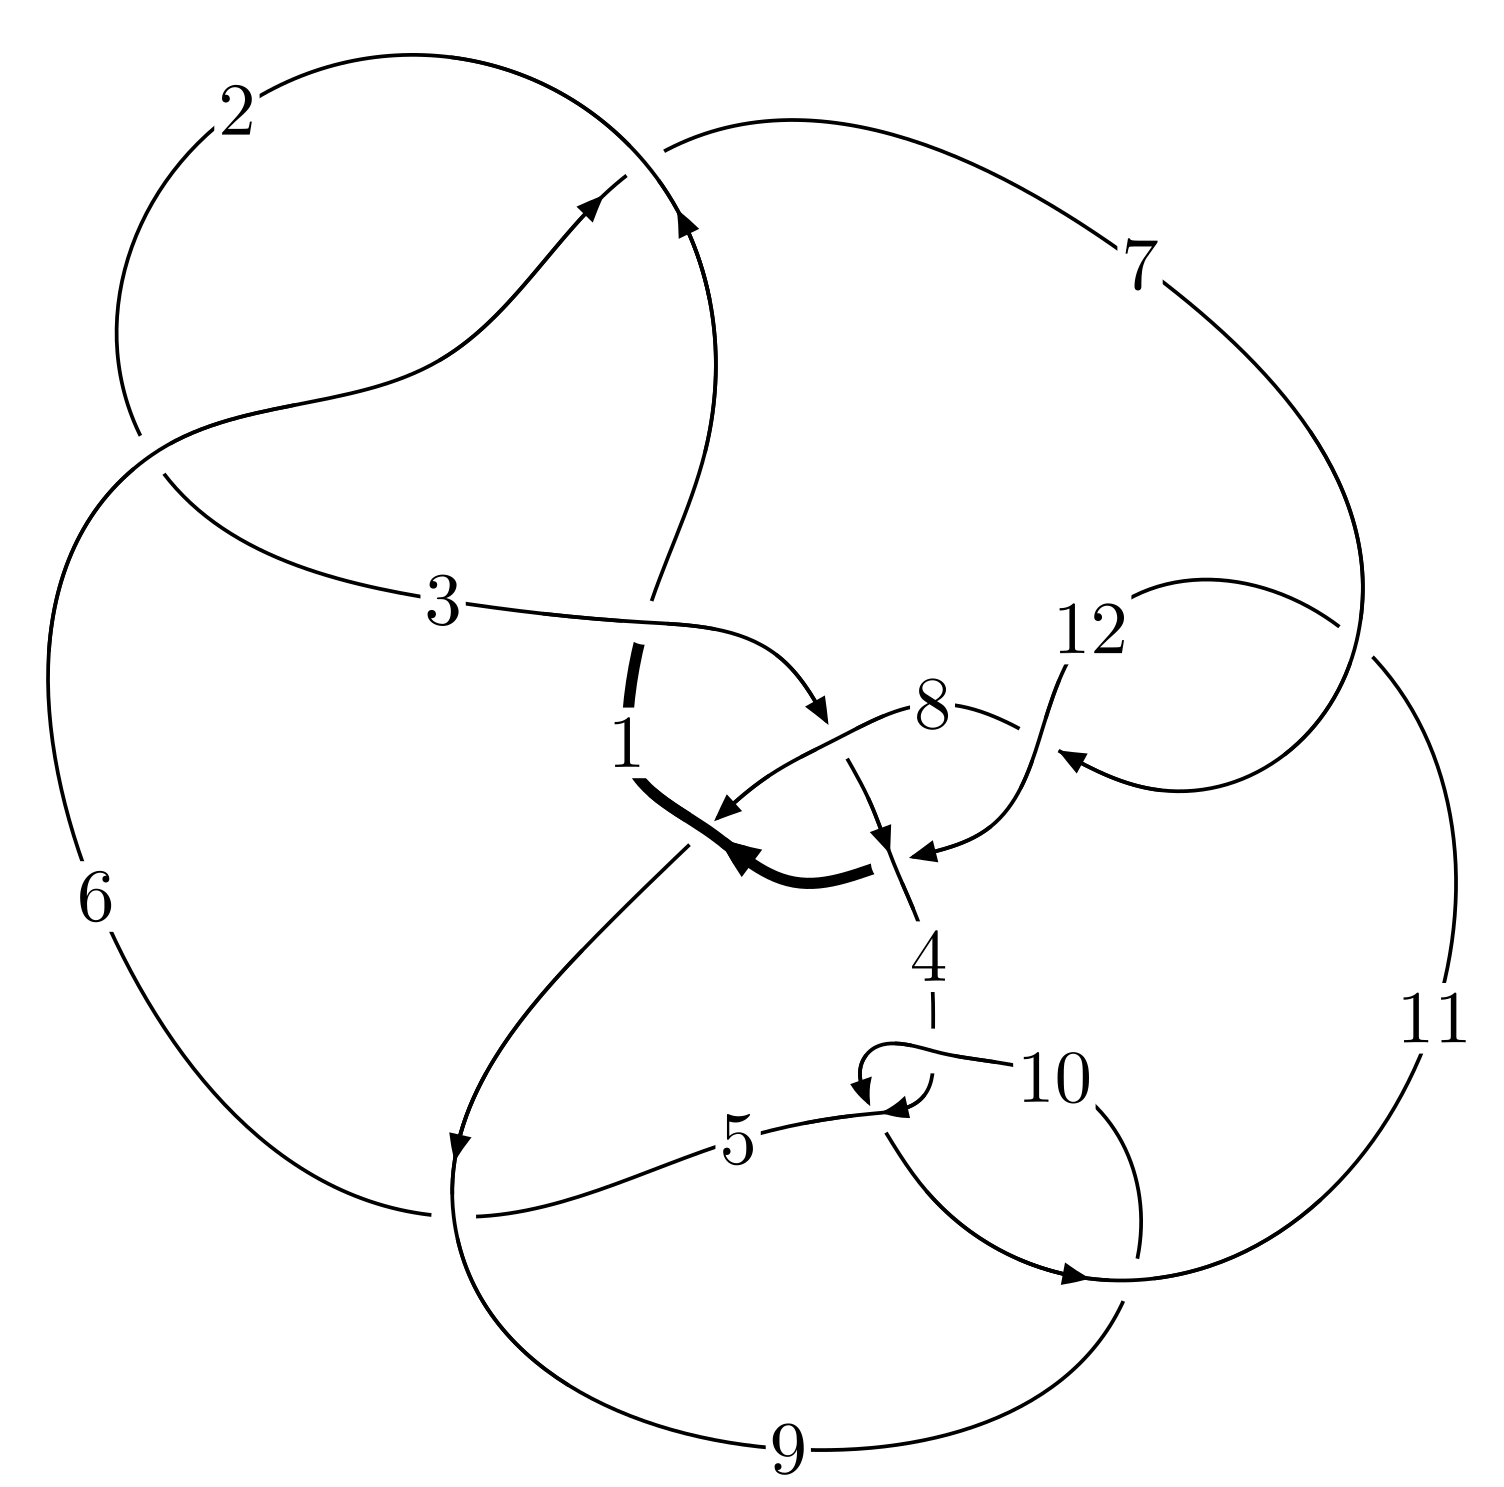
\includegraphics[width=112pt]{../../../GIT/diagram.site/Diagrams/png/1111_12a_0310.png}\\
\ \ \ A knot diagram\footnotemark}&
\allowdisplaybreaks
\textbf{Linearized knot diagam} \\
\cline{2-2}
 &
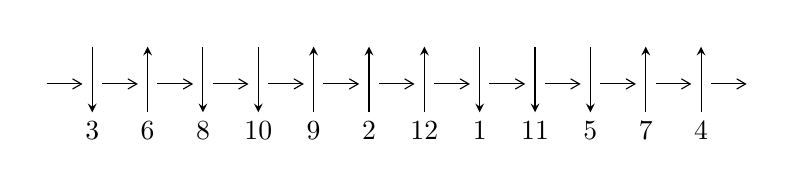
\begin{tikzpicture}[x=20pt, y=17pt]
	% nodes
	\node (C0) at (0, 0) {};
	\node (C1) at (1, 0) {};
	\node (C1U) at (1, +1) {};
	\node (C1D) at (1, -1) {3};

	\node (C2) at (2, 0) {};
	\node (C2U) at (2, +1) {};
	\node (C2D) at (2, -1) {6};

	\node (C3) at (3, 0) {};
	\node (C3U) at (3, +1) {};
	\node (C3D) at (3, -1) {8};

	\node (C4) at (4, 0) {};
	\node (C4U) at (4, +1) {};
	\node (C4D) at (4, -1) {10};

	\node (C5) at (5, 0) {};
	\node (C5U) at (5, +1) {};
	\node (C5D) at (5, -1) {9};

	\node (C6) at (6, 0) {};
	\node (C6U) at (6, +1) {};
	\node (C6D) at (6, -1) {2};

	\node (C7) at (7, 0) {};
	\node (C7U) at (7, +1) {};
	\node (C7D) at (7, -1) {12};

	\node (C8) at (8, 0) {};
	\node (C8U) at (8, +1) {};
	\node (C8D) at (8, -1) {1};

	\node (C9) at (9, 0) {};
	\node (C9U) at (9, +1) {};
	\node (C9D) at (9, -1) {11};

	\node (C10) at (10, 0) {};
	\node (C10U) at (10, +1) {};
	\node (C10D) at (10, -1) {5};

	\node (C11) at (11, 0) {};
	\node (C11U) at (11, +1) {};
	\node (C11D) at (11, -1) {7};

	\node (C12) at (12, 0) {};
	\node (C12U) at (12, +1) {};
	\node (C12D) at (12, -1) {4};
	\node (C13) at (13, 0) {};

	% arrows
	\draw[->,>={angle 60}]
	(C0) edge (C1) (C1) edge (C2) (C2) edge (C3) (C3) edge (C4) (C4) edge (C5) (C5) edge (C6) (C6) edge (C7) (C7) edge (C8) (C8) edge (C9) (C9) edge (C10) (C10) edge (C11) (C11) edge (C12) (C12) edge (C13) ;	\draw[->,>=stealth]
	(C1U) edge (C1D) (C2D) edge (C2U) (C3U) edge (C3D) (C4U) edge (C4D) (C5D) edge (C5U) (C6D) edge (C6U) (C7D) edge (C7U) (C8U) edge (C8D) (C9U) edge (C9D) (C10U) edge (C10D) (C11D) edge (C11U) (C12D) edge (C12U) ;
	\end{tikzpicture} \\
\hhline{~~} \\& 
\textbf{Solving Sequence} \\ \cline{2-2} 
 &
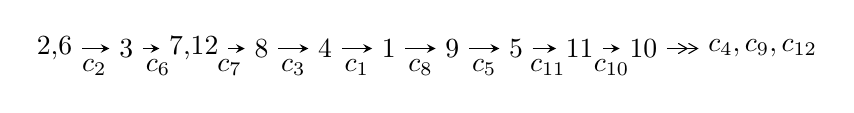
\begin{tikzpicture}[x=23pt, y=7pt]
	% node
	\node (A0) at (-1/8, 0) {2,6};
	\node (A1) at (1, 0) {3};
	\node (A2) at (33/16, 0) {7,12};
	\node (A3) at (25/8, 0) {8};
	\node (A4) at (33/8, 0) {4};
	\node (A5) at (41/8, 0) {1};
	\node (A6) at (49/8, 0) {9};
	\node (A7) at (57/8, 0) {5};
	\node (A8) at (65/8, 0) {11};
	\node (A9) at (73/8, 0) {10};
	\node (C1) at (1/2, -1) {$c_{2}$};
	\node (C2) at (3/2, -1) {$c_{6}$};
	\node (C3) at (21/8, -1) {$c_{7}$};
	\node (C4) at (29/8, -1) {$c_{3}$};
	\node (C5) at (37/8, -1) {$c_{1}$};
	\node (C6) at (45/8, -1) {$c_{8}$};
	\node (C7) at (53/8, -1) {$c_{5}$};
	\node (C8) at (61/8, -1) {$c_{11}$};
	\node (C9) at (69/8, -1) {$c_{10}$};
	\node (A10) at (11, 0) {$c_{4},c_{9},c_{12}$};

	% edge
	\draw[->,>=stealth]	
	(A0) edge (A1) (A1) edge (A2) (A2) edge (A3) (A3) edge (A4) (A4) edge (A5) (A5) edge (A6) (A6) edge (A7) (A7) edge (A8) (A8) edge (A9) ;
	\draw[->>,>={angle 60}]	
	(A9) edge (A10);
\end{tikzpicture} \\ 

\end{tabular} \\

\footnotetext{
The image of knot diagram is generated by the software ``\textbf{Draw programme}" developed by Andrew Bartholomew(\url{http://www.layer8.co.uk/maths/draw/index.htm\#Running-draw}), where we modified some parts for our purpose(\url{https://github.com/CATsTAILs/LinksPainter}).
}\phantom \\ \newline 
\centering \textbf{Ideals for irreducible components\footnotemark of $X_{\text{par}}$} 
 
\begin{align*}
I^u_{1}&=\langle 
2.27433\times10^{354} u^{137}+1.24436\times10^{355} u^{136}+\cdots+1.06021\times10^{355} b-9.00762\times10^{355},\\
\phantom{I^u_{1}}&\phantom{= \langle  }1.69855\times10^{354} u^{137}+8.78430\times10^{354} u^{136}+\cdots+1.06021\times10^{355} a-4.05574\times10^{356},\\
\phantom{I^u_{1}}&\phantom{= \langle  }u^{138}+7 u^{137}+\cdots+1836 u+216\rangle \\
I^u_{2}&=\langle 
7 u^{29}-7 u^{28}+\cdots+b-1,\;6 u^{29}-7 u^{28}+\cdots+a-9,\;u^{30}- u^{29}+\cdots- u+1\rangle \\
I^u_{3}&=\langle 
-5169 a^6 u+14986 a^5 u+\cdots-286138 a+106454,\\
\phantom{I^u_{3}}&\phantom{= \langle  }a^7-2 a^6 u-11 a^5 u+6 a^5+24 a^4 u-38 a^4+4 a^3 u+46 a^3-48 a^2 u-2 a^2+28 a u-25 a- u+6,\;u^2- u+1\rangle \\
\\
\end{align*}
\raggedright * 3 irreducible components of $\dim_{\mathbb{C}}=0$, with total 182 representations.\\
\footnotetext{All coefficients of polynomials are rational numbers. But the coefficients are sometimes approximated in decimal forms when there is not enough margin.}
\newpage
\renewcommand{\arraystretch}{1}
\centering \section*{I. $I^u_{1}= \langle 2.27\times10^{354} u^{137}+1.24\times10^{355} u^{136}+\cdots+1.06\times10^{355} b-9.01\times10^{355},\;1.70\times10^{354} u^{137}+8.78\times10^{354} u^{136}+\cdots+1.06\times10^{355} a-4.06\times10^{356},\;u^{138}+7 u^{137}+\cdots+1836 u+216 \rangle$}
\flushleft \textbf{(i) Arc colorings}\\
\begin{tabular}{m{7pt} m{180pt} m{7pt} m{180pt} }
\flushright $a_{2}=$&$\begin{pmatrix}1\\0\end{pmatrix}$ \\
\flushright $a_{6}=$&$\begin{pmatrix}0\\u\end{pmatrix}$ \\
\flushright $a_{3}=$&$\begin{pmatrix}1\\- u^2\end{pmatrix}$ \\
\flushright $a_{7}=$&$\begin{pmatrix}u\\u\end{pmatrix}$ \\
\flushright $a_{12}=$&$\begin{pmatrix}-0.160209 u^{137}-0.828543 u^{136}+\cdots+203.274 u+38.2541\\-0.214516 u^{137}-1.17370 u^{136}+\cdots+19.3693 u+8.49607\end{pmatrix}$ \\
\flushright $a_{8}=$&$\begin{pmatrix}0.380098 u^{137}+2.08238 u^{136}+\cdots-240.204 u-56.1677\\0.0620701 u^{137}-0.0770345 u^{136}+\cdots-794.079 u-113.783\end{pmatrix}$ \\
\flushright $a_{4}=$&$\begin{pmatrix}0.205743 u^{137}+1.62270 u^{136}+\cdots+376.900 u+42.9007\\0.407264 u^{137}+2.77702 u^{136}+\cdots+574.740 u+61.4601\end{pmatrix}$ \\
\flushright $a_{1}=$&$\begin{pmatrix}u^2+1\\- u^4\end{pmatrix}$ \\
\flushright $a_{9}=$&$\begin{pmatrix}-0.0740279 u^{137}-0.834982 u^{136}+\cdots-801.708 u-118.094\\-0.248617 u^{137}-2.06032 u^{136}+\cdots-1061.70 u-139.977\end{pmatrix}$ \\
\flushright $a_{5}=$&$\begin{pmatrix}0.249137 u^{137}+2.01530 u^{136}+\cdots+1083.50 u+153.271\\0.207662 u^{137}+1.53167 u^{136}+\cdots+417.061 u+47.7159\end{pmatrix}$ \\
\flushright $a_{11}=$&$\begin{pmatrix}-0.147415 u^{137}-0.716549 u^{136}+\cdots+255.807 u+45.8145\\-0.201723 u^{137}-1.06170 u^{136}+\cdots+71.9021 u+16.0565\end{pmatrix}$ \\
\flushright $a_{10}=$&$\begin{pmatrix}-0.231859 u^{137}-2.11061 u^{136}+\cdots-1274.80 u-174.147\\-0.403432 u^{137}-3.02889 u^{136}+\cdots-1012.28 u-119.100\end{pmatrix}$\\&\end{tabular}
\flushleft \textbf{(ii) Obstruction class $= -1$}\\~\\
\flushleft \textbf{(iii) Cusp Shapes $= -0.117732 u^{137}-0.757477 u^{136}+\cdots-388.494 u-88.6881$}\\~\\
\newpage\renewcommand{\arraystretch}{1}
\flushleft \textbf{(iv) u-Polynomials at the component}\newline \\
\begin{tabular}{m{50pt}|m{274pt}}
Crossings & \hspace{64pt}u-Polynomials at each crossing \\
\hline $$\begin{aligned}c_{1}\end{aligned}$$&$\begin{aligned}
&u^{138}+57 u^{137}+\cdots+802224 u+46656
\end{aligned}$\\
\hline $$\begin{aligned}c_{2},c_{6}\end{aligned}$$&$\begin{aligned}
&u^{138}+7 u^{137}+\cdots+1836 u+216
\end{aligned}$\\
\hline $$\begin{aligned}c_{3}\end{aligned}$$&$\begin{aligned}
&u^{138}- u^{137}+\cdots-54398 u+10041
\end{aligned}$\\
\hline $$\begin{aligned}c_{4},c_{10}\end{aligned}$$&$\begin{aligned}
&u^{138}- u^{137}+\cdots-30 u+19
\end{aligned}$\\
\hline $$\begin{aligned}c_{5}\end{aligned}$$&$\begin{aligned}
&u^{138}-3 u^{137}+\cdots-5664770 u+21046851
\end{aligned}$\\
\hline $$\begin{aligned}c_{7},c_{11}\end{aligned}$$&$\begin{aligned}
&u^{138}-3 u^{137}+\cdots+378940 u+19571
\end{aligned}$\\
\hline $$\begin{aligned}c_{8}\end{aligned}$$&$\begin{aligned}
&u^{138}+u^{137}+\cdots-50 u+1
\end{aligned}$\\
\hline $$\begin{aligned}c_{9}\end{aligned}$$&$\begin{aligned}
&u^{138}+71 u^{137}+\cdots+3712 u+361
\end{aligned}$\\
\hline $$\begin{aligned}c_{12}\end{aligned}$$&$\begin{aligned}
&u^{138}+13 u^{137}+\cdots-310 u+77
\end{aligned}$\\
\hline
\end{tabular}\\~\\
\newpage\renewcommand{\arraystretch}{1}
\flushleft \textbf{(v) Riley Polynomials at the component}\newline \\
\begin{tabular}{m{50pt}|m{274pt}}
Crossings & \hspace{64pt}Riley Polynomials at each crossing \\
\hline $$\begin{aligned}c_{1}\end{aligned}$$&$\begin{aligned}
&y^{138}+57 y^{137}+\cdots+94721944320 y+2176782336
\end{aligned}$\\
\hline $$\begin{aligned}c_{2},c_{6}\end{aligned}$$&$\begin{aligned}
&y^{138}+57 y^{137}+\cdots+802224 y+46656
\end{aligned}$\\
\hline $$\begin{aligned}c_{3}\end{aligned}$$&$\begin{aligned}
&y^{138}+31 y^{137}+\cdots+4830062936 y+100821681
\end{aligned}$\\
\hline $$\begin{aligned}c_{4},c_{10}\end{aligned}$$&$\begin{aligned}
&y^{138}-71 y^{137}+\cdots-3712 y+361
\end{aligned}$\\
\hline $$\begin{aligned}c_{5}\end{aligned}$$&$\begin{aligned}
&y^{138}+45 y^{137}+\cdots+9711800845573616 y+442969937016201
\end{aligned}$\\
\hline $$\begin{aligned}c_{7},c_{11}\end{aligned}$$&$\begin{aligned}
&y^{138}-101 y^{137}+\cdots-89234996574 y+383024041
\end{aligned}$\\
\hline $$\begin{aligned}c_{8}\end{aligned}$$&$\begin{aligned}
&y^{138}-3 y^{137}+\cdots-576 y+1
\end{aligned}$\\
\hline $$\begin{aligned}c_{9}\end{aligned}$$&$\begin{aligned}
&y^{138}+13 y^{137}+\cdots+3788760 y+130321
\end{aligned}$\\
\hline $$\begin{aligned}c_{12}\end{aligned}$$&$\begin{aligned}
&y^{138}-11 y^{137}+\cdots-433668 y+5929
\end{aligned}$\\
\hline
\end{tabular}\\~\\
\newpage\flushleft \textbf{(vi) Complex Volumes and Cusp Shapes}
$$\begin{array}{c|c|c}  
\text{Solutions to }I^u_{1}& \I (\text{vol} + \sqrt{-1}CS) & \text{Cusp shape}\\
 \hline 
\begin{aligned}
u &= \phantom{-}0.323280 + 0.949945 I \\
a &= \phantom{-}0.483460 + 0.228596 I \\
b &= \phantom{-}0.108033 - 1.022500 I\end{aligned}
 & -0.19526 - 4.44594 I & \phantom{-0.000000 } 0 \\ \hline\begin{aligned}
u &= \phantom{-}0.323280 - 0.949945 I \\
a &= \phantom{-}0.483460 - 0.228596 I \\
b &= \phantom{-}0.108033 + 1.022500 I\end{aligned}
 & -0.19526 + 4.44594 I & \phantom{-0.000000 } 0 \\ \hline\begin{aligned}
u &= \phantom{-}0.760685 + 0.685269 I \\
a &= -1.33908 - 1.81762 I \\
b &= -2.12515 - 0.84369 I\end{aligned}
 & \phantom{-}6.65208 + 0.07508 I & \phantom{-0.000000 } 0 \\ \hline\begin{aligned}
u &= \phantom{-}0.760685 - 0.685269 I \\
a &= -1.33908 + 1.81762 I \\
b &= -2.12515 + 0.84369 I\end{aligned}
 & \phantom{-}6.65208 - 0.07508 I & \phantom{-0.000000 } 0 \\ \hline\begin{aligned}
u &= \phantom{-}0.801138 + 0.553328 I \\
a &= \phantom{-}0.463585 + 0.478130 I \\
b &= -0.213753 - 0.624818 I\end{aligned}
 & -1.68579 - 7.34118 I & \phantom{-0.000000 } 0 \\ \hline\begin{aligned}
u &= \phantom{-}0.801138 - 0.553328 I \\
a &= \phantom{-}0.463585 - 0.478130 I \\
b &= -0.213753 + 0.624818 I\end{aligned}
 & -1.68579 + 7.34118 I & \phantom{-0.000000 } 0 \\ \hline\begin{aligned}
u &= \phantom{-}0.875262 + 0.421574 I \\
a &= -0.58037 - 1.80626 I \\
b &= -1.49669 - 0.75441 I\end{aligned}
 & \phantom{-}0.30791 - 5.36080 I & \phantom{-0.000000 } 0 \\ \hline\begin{aligned}
u &= \phantom{-}0.875262 - 0.421574 I \\
a &= -0.58037 + 1.80626 I \\
b &= -1.49669 + 0.75441 I\end{aligned}
 & \phantom{-}0.30791 + 5.36080 I & \phantom{-0.000000 } 0 \\ \hline\begin{aligned}
u &= -0.831916 + 0.626363 I \\
a &= -1.06965 + 1.74488 I \\
b &= -1.90743 + 0.75097 I\end{aligned}
 & \phantom{-}7.31279 + 5.38938 I & \phantom{-0.000000 } 0 \\ \hline\begin{aligned}
u &= -0.831916 - 0.626363 I \\
a &= -1.06965 - 1.74488 I \\
b &= -1.90743 - 0.75097 I\end{aligned}
 & \phantom{-}7.31279 - 5.38938 I & \phantom{-0.000000 } 0\\
 \hline 
 \end{array}$$\newpage$$\begin{array}{c|c|c}  
\text{Solutions to }I^u_{1}& \I (\text{vol} + \sqrt{-1}CS) & \text{Cusp shape}\\
 \hline 
\begin{aligned}
u &= -0.593104 + 0.751298 I \\
a &= \phantom{-}1.06027 - 2.02579 I \\
b &= \phantom{-}1.52125 - 0.44292 I\end{aligned}
 & \phantom{-}4.36335 + 0.38616 I & \phantom{-0.000000 } 0 \\ \hline\begin{aligned}
u &= -0.593104 - 0.751298 I \\
a &= \phantom{-}1.06027 + 2.02579 I \\
b &= \phantom{-}1.52125 + 0.44292 I\end{aligned}
 & \phantom{-}4.36335 - 0.38616 I & \phantom{-0.000000 } 0 \\ \hline\begin{aligned}
u &= \phantom{-}0.330124 + 0.999756 I \\
a &= \phantom{-}0.542401 + 0.642123 I \\
b &= \phantom{-}0.35058 + 1.43107 I\end{aligned}
 & -0.419083 + 1.060100 I & \phantom{-0.000000 } 0 \\ \hline\begin{aligned}
u &= \phantom{-}0.330124 - 0.999756 I \\
a &= \phantom{-}0.542401 - 0.642123 I \\
b &= \phantom{-}0.35058 - 1.43107 I\end{aligned}
 & -0.419083 - 1.060100 I & \phantom{-0.000000 } 0 \\ \hline\begin{aligned}
u &= -0.480691 + 0.939248 I \\
a &= -2.87238 + 2.39939 I \\
b &= -3.46961 + 1.69138 I\end{aligned}
 & -4.42962 - 6.92429 I & \phantom{-0.000000 } 0 \\ \hline\begin{aligned}
u &= -0.480691 - 0.939248 I \\
a &= -2.87238 - 2.39939 I \\
b &= -3.46961 - 1.69138 I\end{aligned}
 & -4.42962 + 6.92429 I & \phantom{-0.000000 } 0 \\ \hline\begin{aligned}
u &= -0.439143 + 0.816060 I \\
a &= -2.69054 + 3.08949 I \\
b &= -3.16623 + 2.24819 I\end{aligned}
 & -3.95035 + 3.15119 I & \phantom{-0.000000 } 0 \\ \hline\begin{aligned}
u &= -0.439143 - 0.816060 I \\
a &= -2.69054 - 3.08949 I \\
b &= -3.16623 - 2.24819 I\end{aligned}
 & -3.95035 - 3.15119 I & \phantom{-0.000000 } 0 \\ \hline\begin{aligned}
u &= -0.951536 + 0.502856 I \\
a &= -0.70754 + 1.62353 I \\
b &= -1.61602 + 0.61146 I\end{aligned}
 & \phantom{-}5.33287 + 8.32927 I & \phantom{-0.000000 } 0 \\ \hline\begin{aligned}
u &= -0.951536 - 0.502856 I \\
a &= -0.70754 - 1.62353 I \\
b &= -1.61602 - 0.61146 I\end{aligned}
 & \phantom{-}5.33287 - 8.32927 I & \phantom{-0.000000 } 0\\
 \hline 
 \end{array}$$\newpage$$\begin{array}{c|c|c}  
\text{Solutions to }I^u_{1}& \I (\text{vol} + \sqrt{-1}CS) & \text{Cusp shape}\\
 \hline 
\begin{aligned}
u &= -0.399085 + 1.001540 I \\
a &= \phantom{-}0.837137 + 1.011990 I \\
b &= \phantom{-}1.013180 + 0.120356 I\end{aligned}
 & -4.66972 + 1.37466 I & \phantom{-0.000000 } 0 \\ \hline\begin{aligned}
u &= -0.399085 - 1.001540 I \\
a &= \phantom{-}0.837137 - 1.011990 I \\
b &= \phantom{-}1.013180 - 0.120356 I\end{aligned}
 & -4.66972 - 1.37466 I & \phantom{-0.000000 } 0 \\ \hline\begin{aligned}
u &= -0.090055 + 1.088100 I \\
a &= -0.338874 + 0.955777 I \\
b &= -1.070320 + 0.722200 I\end{aligned}
 & -4.30114 + 1.33462 I & \phantom{-0.000000 } 0 \\ \hline\begin{aligned}
u &= -0.090055 - 1.088100 I \\
a &= -0.338874 - 0.955777 I \\
b &= -1.070320 - 0.722200 I\end{aligned}
 & -4.30114 - 1.33462 I & \phantom{-0.000000 } 0 \\ \hline\begin{aligned}
u &= \phantom{-}1.030790 + 0.361032 I \\
a &= \phantom{-}0.523241 + 1.008720 I \\
b &= \phantom{-}1.50088 + 0.65091 I\end{aligned}
 & \phantom{-}5.25592 + 1.03879 I & \phantom{-0.000000 } 0 \\ \hline\begin{aligned}
u &= \phantom{-}1.030790 - 0.361032 I \\
a &= \phantom{-}0.523241 - 1.008720 I \\
b &= \phantom{-}1.50088 - 0.65091 I\end{aligned}
 & \phantom{-}5.25592 - 1.03879 I & \phantom{-0.000000 } 0 \\ \hline\begin{aligned}
u &= -0.719777 + 0.821692 I \\
a &= \phantom{-}0.94526 - 1.71005 I \\
b &= \phantom{-}1.76139 - 0.43491 I\end{aligned}
 & \phantom{-}5.28806 - 1.39704 I & \phantom{-0.000000 } 0 \\ \hline\begin{aligned}
u &= -0.719777 - 0.821692 I \\
a &= \phantom{-}0.94526 + 1.71005 I \\
b &= \phantom{-}1.76139 + 0.43491 I\end{aligned}
 & \phantom{-}5.28806 + 1.39704 I & \phantom{-0.000000 } 0 \\ \hline\begin{aligned}
u &= -0.619725 + 0.658570 I \\
a &= \phantom{-}0.442655 - 0.650121 I \\
b &= -0.329622 - 0.326393 I\end{aligned}
 & -1.96482 + 2.30501 I & \phantom{-0.000000 } 0 \\ \hline\begin{aligned}
u &= -0.619725 - 0.658570 I \\
a &= \phantom{-}0.442655 + 0.650121 I \\
b &= -0.329622 + 0.326393 I\end{aligned}
 & -1.96482 - 2.30501 I & \phantom{-0.000000 } 0\\
 \hline 
 \end{array}$$\newpage$$\begin{array}{c|c|c}  
\text{Solutions to }I^u_{1}& \I (\text{vol} + \sqrt{-1}CS) & \text{Cusp shape}\\
 \hline 
\begin{aligned}
u &= -0.719423 + 0.545668 I \\
a &= \phantom{-}0.490330 - 0.445730 I \\
b &= -0.125810 + 0.613284 I\end{aligned}
 & \phantom{-}0.70027 + 2.74370 I & \phantom{-0.000000 } 0 \\ \hline\begin{aligned}
u &= -0.719423 - 0.545668 I \\
a &= \phantom{-}0.490330 + 0.445730 I \\
b &= -0.125810 - 0.613284 I\end{aligned}
 & \phantom{-}0.70027 - 2.74370 I & \phantom{-0.000000 } 0 \\ \hline\begin{aligned}
u &= -0.584908 + 0.928785 I \\
a &= \phantom{-}0.854248 + 0.679562 I \\
b &= \phantom{-}1.013770 - 0.006712 I\end{aligned}
 & -2.71118 - 7.05562 I & \phantom{-0.000000 } 0 \\ \hline\begin{aligned}
u &= -0.584908 - 0.928785 I \\
a &= \phantom{-}0.854248 - 0.679562 I \\
b &= \phantom{-}1.013770 + 0.006712 I\end{aligned}
 & -2.71118 + 7.05562 I & \phantom{-0.000000 } 0 \\ \hline\begin{aligned}
u &= -0.597159 + 0.921827 I \\
a &= \phantom{-}1.14235 - 1.50319 I \\
b &= \phantom{-}2.40530 - 0.83158 I\end{aligned}
 & \phantom{-}3.82844 - 5.11364 I & \phantom{-0.000000 } 0 \\ \hline\begin{aligned}
u &= -0.597159 - 0.921827 I \\
a &= \phantom{-}1.14235 + 1.50319 I \\
b &= \phantom{-}2.40530 + 0.83158 I\end{aligned}
 & \phantom{-}3.82844 + 5.11364 I & \phantom{-0.000000 } 0 \\ \hline\begin{aligned}
u &= -1.078680 + 0.229525 I \\
a &= \phantom{-}0.482278 - 0.895697 I \\
b &= \phantom{-}1.41770 - 0.58682 I\end{aligned}
 & \phantom{-}3.27001 + 3.57478 I & \phantom{-0.000000 } 0 \\ \hline\begin{aligned}
u &= -1.078680 - 0.229525 I \\
a &= \phantom{-}0.482278 + 0.895697 I \\
b &= \phantom{-}1.41770 + 0.58682 I\end{aligned}
 & \phantom{-}3.27001 - 3.57478 I & \phantom{-0.000000 } 0 \\ \hline\begin{aligned}
u &= \phantom{-}0.996646 + 0.479594 I \\
a &= -0.64453 - 1.55949 I \\
b &= -1.56709 - 0.55145 I\end{aligned}
 & \phantom{-}2.91389 - 13.58860 I & \phantom{-0.000000 } 0 \\ \hline\begin{aligned}
u &= \phantom{-}0.996646 - 0.479594 I \\
a &= -0.64453 + 1.55949 I \\
b &= -1.56709 + 0.55145 I\end{aligned}
 & \phantom{-}2.91389 + 13.58860 I & \phantom{-0.000000 } 0\\
 \hline 
 \end{array}$$\newpage$$\begin{array}{c|c|c}  
\text{Solutions to }I^u_{1}& \I (\text{vol} + \sqrt{-1}CS) & \text{Cusp shape}\\
 \hline 
\begin{aligned}
u &= -0.570025 + 0.950620 I \\
a &= -0.389622 - 0.531561 I \\
b &= \phantom{-}0.572161 - 0.766847 I\end{aligned}
 & \phantom{-}0.86560 - 6.38011 I & \phantom{-0.000000 } 0 \\ \hline\begin{aligned}
u &= -0.570025 - 0.950620 I \\
a &= -0.389622 + 0.531561 I \\
b &= \phantom{-}0.572161 + 0.766847 I\end{aligned}
 & \phantom{-}0.86560 + 6.38011 I & \phantom{-0.000000 } 0 \\ \hline\begin{aligned}
u &= \phantom{-}0.548997 + 0.698275 I \\
a &= \phantom{-}1.08824 + 2.19982 I \\
b &= \phantom{-}1.42208 + 0.39958 I\end{aligned}
 & \phantom{-}2.21535 - 5.27635 I & \phantom{-0.000000 } 0 \\ \hline\begin{aligned}
u &= \phantom{-}0.548997 - 0.698275 I \\
a &= \phantom{-}1.08824 - 2.19982 I \\
b &= \phantom{-}1.42208 - 0.39958 I\end{aligned}
 & \phantom{-}2.21535 + 5.27635 I & \phantom{-0.000000 } 0 \\ \hline\begin{aligned}
u &= \phantom{-}0.564026 + 0.968718 I \\
a &= \phantom{-}1.23961 + 1.45847 I \\
b &= \phantom{-}2.53662 + 0.81384 I\end{aligned}
 & \phantom{-}1.34717 + 9.77817 I & \phantom{-0.000000 } 0 \\ \hline\begin{aligned}
u &= \phantom{-}0.564026 - 0.968718 I \\
a &= \phantom{-}1.23961 - 1.45847 I \\
b &= \phantom{-}2.53662 - 0.81384 I\end{aligned}
 & \phantom{-}1.34717 - 9.77817 I & \phantom{-0.000000 } 0 \\ \hline\begin{aligned}
u &= -0.266933 + 1.089480 I \\
a &= \phantom{-}0.411875 - 0.354237 I \\
b &= \phantom{-}0.322519 - 1.267820 I\end{aligned}
 & -3.17108 + 3.91786 I & \phantom{-0.000000 } 0 \\ \hline\begin{aligned}
u &= -0.266933 - 1.089480 I \\
a &= \phantom{-}0.411875 + 0.354237 I \\
b &= \phantom{-}0.322519 + 1.267820 I\end{aligned}
 & -3.17108 - 3.91786 I & \phantom{-0.000000 } 0 \\ \hline\begin{aligned}
u &= -0.164916 + 0.860488 I \\
a &= \phantom{-}0.599830 - 0.193590 I \\
b &= \phantom{-}0.214859 + 0.999503 I\end{aligned}
 & \phantom{-}1.38836 + 0.83662 I & \phantom{-0.000000 } 0 \\ \hline\begin{aligned}
u &= -0.164916 - 0.860488 I \\
a &= \phantom{-}0.599830 + 0.193590 I \\
b &= \phantom{-}0.214859 - 0.999503 I\end{aligned}
 & \phantom{-}1.38836 - 0.83662 I & \phantom{-0.000000 } 0\\
 \hline 
 \end{array}$$\newpage$$\begin{array}{c|c|c}  
\text{Solutions to }I^u_{1}& \I (\text{vol} + \sqrt{-1}CS) & \text{Cusp shape}\\
 \hline 
\begin{aligned}
u &= -0.520582 + 0.702605 I \\
a &= \phantom{-}0.478088 - 0.364264 I \\
b &= \phantom{-}0.037388 + 0.812572 I\end{aligned}
 & \phantom{-}1.66387 + 1.91116 I & \phantom{-0.000000 } 0 \\ \hline\begin{aligned}
u &= -0.520582 - 0.702605 I \\
a &= \phantom{-}0.478088 + 0.364264 I \\
b &= \phantom{-}0.037388 - 0.812572 I\end{aligned}
 & \phantom{-}1.66387 - 1.91116 I & \phantom{-0.000000 } 0 \\ \hline\begin{aligned}
u &= \phantom{-}0.042173 + 1.126530 I \\
a &= -0.531546 - 1.174140 I \\
b &= -1.24634 - 0.96390 I\end{aligned}
 & -7.35847 - 5.89473 I & \phantom{-0.000000 } 0 \\ \hline\begin{aligned}
u &= \phantom{-}0.042173 - 1.126530 I \\
a &= -0.531546 + 1.174140 I \\
b &= -1.24634 + 0.96390 I\end{aligned}
 & -7.35847 + 5.89473 I & \phantom{-0.000000 } 0 \\ \hline\begin{aligned}
u &= \phantom{-}0.763284 + 0.408398 I \\
a &= \phantom{-}0.550601 + 0.516451 I \\
b &= -0.194341 - 0.457642 I\end{aligned}
 & -3.05106 + 0.17655 I & \phantom{-0.000000 } 0 \\ \hline\begin{aligned}
u &= \phantom{-}0.763284 - 0.408398 I \\
a &= \phantom{-}0.550601 - 0.516451 I \\
b &= -0.194341 + 0.457642 I\end{aligned}
 & -3.05106 - 0.17655 I & \phantom{-0.000000 } 0 \\ \hline\begin{aligned}
u &= -0.407542 + 1.071160 I \\
a &= -0.659775 - 0.129486 I \\
b &= -1.298270 - 0.503505 I\end{aligned}
 & -5.09715 - 2.91594 I & \phantom{-0.000000 } 0 \\ \hline\begin{aligned}
u &= -0.407542 - 1.071160 I \\
a &= -0.659775 + 0.129486 I \\
b &= -1.298270 + 0.503505 I\end{aligned}
 & -5.09715 + 2.91594 I & \phantom{-0.000000 } 0 \\ \hline\begin{aligned}
u &= \phantom{-}0.781994 + 0.841327 I \\
a &= \phantom{-}0.86760 + 1.57118 I \\
b &= \phantom{-}1.89224 + 0.39385 I\end{aligned}
 & \phantom{-}3.94008 + 5.80075 I & \phantom{-0.000000 } 0 \\ \hline\begin{aligned}
u &= \phantom{-}0.781994 - 0.841327 I \\
a &= \phantom{-}0.86760 - 1.57118 I \\
b &= \phantom{-}1.89224 - 0.39385 I\end{aligned}
 & \phantom{-}3.94008 - 5.80075 I & \phantom{-0.000000 } 0\\
 \hline 
 \end{array}$$\newpage$$\begin{array}{c|c|c}  
\text{Solutions to }I^u_{1}& \I (\text{vol} + \sqrt{-1}CS) & \text{Cusp shape}\\
 \hline 
\begin{aligned}
u &= \phantom{-}0.511774 + 1.029730 I \\
a &= -1.36061 + 0.55979 I \\
b &= -1.96792 + 1.14221 I\end{aligned}
 & \phantom{-}0.75603 + 5.26566 I & \phantom{-0.000000 } 0 \\ \hline\begin{aligned}
u &= \phantom{-}0.511774 - 1.029730 I \\
a &= -1.36061 - 0.55979 I \\
b &= -1.96792 - 1.14221 I\end{aligned}
 & \phantom{-}0.75603 - 5.26566 I & \phantom{-0.000000 } 0 \\ \hline\begin{aligned}
u &= \phantom{-}0.142818 + 1.148110 I \\
a &= -0.570941 - 0.752056 I \\
b &= -1.32602 - 0.52170 I\end{aligned}
 & -8.04836 + 2.50326 I & \phantom{-0.000000 } 0 \\ \hline\begin{aligned}
u &= \phantom{-}0.142818 - 1.148110 I \\
a &= -0.570941 + 0.752056 I \\
b &= -1.32602 + 0.52170 I\end{aligned}
 & -8.04836 - 2.50326 I & \phantom{-0.000000 } 0 \\ \hline\begin{aligned}
u &= -0.723297 + 0.906738 I \\
a &= \phantom{-}0.98176 - 1.42393 I \\
b &= \phantom{-}2.19296 - 0.62674 I\end{aligned}
 & \phantom{-}5.04090 - 4.11717 I & \phantom{-0.000000 } 0 \\ \hline\begin{aligned}
u &= -0.723297 - 0.906738 I \\
a &= \phantom{-}0.98176 + 1.42393 I \\
b &= \phantom{-}2.19296 + 0.62674 I\end{aligned}
 & \phantom{-}5.04090 + 4.11717 I & \phantom{-0.000000 } 0 \\ \hline\begin{aligned}
u &= -0.422900 + 1.101240 I \\
a &= \phantom{-}0.103900 - 0.497296 I \\
b &= \phantom{-}0.213509 - 1.160610 I\end{aligned}
 & -4.99467 - 4.32481 I & \phantom{-0.000000 } 0 \\ \hline\begin{aligned}
u &= -0.422900 - 1.101240 I \\
a &= \phantom{-}0.103900 + 0.497296 I \\
b &= \phantom{-}0.213509 + 1.160610 I\end{aligned}
 & -4.99467 + 4.32481 I & \phantom{-0.000000 } 0 \\ \hline\begin{aligned}
u &= \phantom{-}0.663826 + 0.980340 I \\
a &= -1.71885 - 2.03719 I \\
b &= -2.54130 - 1.27181 I\end{aligned}
 & \phantom{-}5.74476 + 5.32645 I & \phantom{-0.000000 } 0 \\ \hline\begin{aligned}
u &= \phantom{-}0.663826 - 0.980340 I \\
a &= -1.71885 + 2.03719 I \\
b &= -2.54130 + 1.27181 I\end{aligned}
 & \phantom{-}5.74476 - 5.32645 I & \phantom{-0.000000 } 0\\
 \hline 
 \end{array}$$\newpage$$\begin{array}{c|c|c}  
\text{Solutions to }I^u_{1}& \I (\text{vol} + \sqrt{-1}CS) & \text{Cusp shape}\\
 \hline 
\begin{aligned}
u &= \phantom{-}0.777023 + 0.911427 I \\
a &= \phantom{-}0.92311 + 1.40843 I \\
b &= \phantom{-}2.12712 + 0.48932 I\end{aligned}
 & \phantom{-}3.73479 + 0.06546 I & \phantom{-0.000000 } 0 \\ \hline\begin{aligned}
u &= \phantom{-}0.777023 - 0.911427 I \\
a &= \phantom{-}0.92311 - 1.40843 I \\
b &= \phantom{-}2.12712 - 0.48932 I\end{aligned}
 & \phantom{-}3.73479 - 0.06546 I & \phantom{-0.000000 } 0 \\ \hline\begin{aligned}
u &= -0.538027 + 1.072180 I \\
a &= -1.363050 - 0.168615 I \\
b &= -2.04684 - 0.74021 I\end{aligned}
 & -1.44300 - 11.00510 I & \phantom{-0.000000 } 0 \\ \hline\begin{aligned}
u &= -0.538027 - 1.072180 I \\
a &= -1.363050 + 0.168615 I \\
b &= -2.04684 + 0.74021 I\end{aligned}
 & -1.44300 + 11.00510 I & \phantom{-0.000000 } 0 \\ \hline\begin{aligned}
u &= -0.087234 + 0.792376 I \\
a &= \phantom{-}0.748133 + 0.385415 I \\
b &= -0.155133 + 0.214003 I\end{aligned}
 & -1.50983 + 1.66829 I & \phantom{-0.000000 } 0 \\ \hline\begin{aligned}
u &= -0.087234 - 0.792376 I \\
a &= \phantom{-}0.748133 - 0.385415 I \\
b &= -0.155133 - 0.214003 I\end{aligned}
 & -1.50983 - 1.66829 I & \phantom{-0.000000 } 0 \\ \hline\begin{aligned}
u &= \phantom{-}0.553269 + 1.075870 I \\
a &= \phantom{-}0.042987 + 0.687902 I \\
b &= \phantom{-}0.017960 + 0.385961 I\end{aligned}
 & \phantom{-}0.44272 + 3.44736 I & \phantom{-0.000000 } 0 \\ \hline\begin{aligned}
u &= \phantom{-}0.553269 - 1.075870 I \\
a &= \phantom{-}0.042987 - 0.687902 I \\
b &= \phantom{-}0.017960 - 0.385961 I\end{aligned}
 & \phantom{-}0.44272 - 3.44736 I & \phantom{-0.000000 } 0 \\ \hline\begin{aligned}
u &= \phantom{-}0.631032 + 0.468979 I \\
a &= \phantom{-}0.573629 - 0.179992 I \\
b &= \phantom{-}0.688767 - 0.226916 I\end{aligned}
 & \phantom{-}2.24325 + 1.22888 I & \phantom{-0.000000 } 0 \\ \hline\begin{aligned}
u &= \phantom{-}0.631032 - 0.468979 I \\
a &= \phantom{-}0.573629 + 0.179992 I \\
b &= \phantom{-}0.688767 + 0.226916 I\end{aligned}
 & \phantom{-}2.24325 - 1.22888 I & \phantom{-0.000000 } 0\\
 \hline 
 \end{array}$$\newpage$$\begin{array}{c|c|c}  
\text{Solutions to }I^u_{1}& \I (\text{vol} + \sqrt{-1}CS) & \text{Cusp shape}\\
 \hline 
\begin{aligned}
u &= -0.636133 + 1.047580 I \\
a &= -0.282943 - 0.363157 I \\
b &= \phantom{-}0.565230 - 0.933050 I\end{aligned}
 & -0.77613 - 7.96761 I & \phantom{-0.000000 } 0 \\ \hline\begin{aligned}
u &= -0.636133 - 1.047580 I \\
a &= -0.282943 + 0.363157 I \\
b &= \phantom{-}0.565230 + 0.933050 I\end{aligned}
 & -0.77613 + 7.96761 I & \phantom{-0.000000 } 0 \\ \hline\begin{aligned}
u &= -0.688707 + 1.031180 I \\
a &= -1.67633 + 1.76406 I \\
b &= -2.54328 + 1.03588 I\end{aligned}
 & \phantom{-}6.07304 - 11.06380 I & \phantom{-0.000000 } 0 \\ \hline\begin{aligned}
u &= -0.688707 - 1.031180 I \\
a &= -1.67633 - 1.76406 I \\
b &= -2.54328 - 1.03588 I\end{aligned}
 & \phantom{-}6.07304 + 11.06380 I & \phantom{-0.000000 } 0 \\ \hline\begin{aligned}
u &= \phantom{-}1.075570 + 0.620271 I \\
a &= \phantom{-}0.745044 + 1.085970 I \\
b &= \phantom{-}1.68617 + 0.62259 I\end{aligned}
 & \phantom{-}5.62213 + 2.48282 I & \phantom{-0.000000 } 0 \\ \hline\begin{aligned}
u &= \phantom{-}1.075570 - 0.620271 I \\
a &= \phantom{-}0.745044 - 1.085970 I \\
b &= \phantom{-}1.68617 - 0.62259 I\end{aligned}
 & \phantom{-}5.62213 - 2.48282 I & \phantom{-0.000000 } 0 \\ \hline\begin{aligned}
u &= \phantom{-}0.597712 + 1.096410 I \\
a &= -0.192094 + 0.367419 I \\
b &= \phantom{-}0.493155 + 0.982708 I\end{aligned}
 & -5.07060 + 4.96676 I & \phantom{-0.000000 } 0 \\ \hline\begin{aligned}
u &= \phantom{-}0.597712 - 1.096410 I \\
a &= -0.192094 - 0.367419 I \\
b &= \phantom{-}0.493155 - 0.982708 I\end{aligned}
 & -5.07060 - 4.96676 I & \phantom{-0.000000 } 0 \\ \hline\begin{aligned}
u &= \phantom{-}0.664444 + 1.069000 I \\
a &= -0.276412 + 0.314716 I \\
b &= \phantom{-}0.588337 + 0.971677 I\end{aligned}
 & -3.23471 + 12.86910 I & \phantom{-0.000000 } 0 \\ \hline\begin{aligned}
u &= \phantom{-}0.664444 - 1.069000 I \\
a &= -0.276412 - 0.314716 I \\
b &= \phantom{-}0.588337 - 0.971677 I\end{aligned}
 & -3.23471 - 12.86910 I & \phantom{-0.000000 } 0\\
 \hline 
 \end{array}$$\newpage$$\begin{array}{c|c|c}  
\text{Solutions to }I^u_{1}& \I (\text{vol} + \sqrt{-1}CS) & \text{Cusp shape}\\
 \hline 
\begin{aligned}
u &= \phantom{-}0.302296 + 1.246920 I \\
a &= \phantom{-}0.094735 + 0.895059 I \\
b &= \phantom{-}0.425561 + 0.194124 I\end{aligned}
 & -0.16648 + 5.11992 I & \phantom{-0.000000 } 0 \\ \hline\begin{aligned}
u &= \phantom{-}0.302296 - 1.246920 I \\
a &= \phantom{-}0.094735 - 0.895059 I \\
b &= \phantom{-}0.425561 - 0.194124 I\end{aligned}
 & -0.16648 - 5.11992 I & \phantom{-0.000000 } 0 \\ \hline\begin{aligned}
u &= \phantom{-}0.074324 + 1.293770 I \\
a &= \phantom{-}0.338939 - 0.984478 I \\
b &= \phantom{-}0.696779 - 0.093011 I\end{aligned}
 & -5.68762 - 2.51487 I & \phantom{-0.000000 } 0 \\ \hline\begin{aligned}
u &= \phantom{-}0.074324 - 1.293770 I \\
a &= \phantom{-}0.338939 + 0.984478 I \\
b &= \phantom{-}0.696779 + 0.093011 I\end{aligned}
 & -5.68762 + 2.51487 I & \phantom{-0.000000 } 0 \\ \hline\begin{aligned}
u &= \phantom{-}0.645555 + 1.129550 I \\
a &= -1.88462 - 1.37420 I \\
b &= -2.76464 - 0.75003 I\end{aligned}
 & -1.80938 + 10.97010 I & \phantom{-0.000000 } 0 \\ \hline\begin{aligned}
u &= \phantom{-}0.645555 - 1.129550 I \\
a &= -1.88462 + 1.37420 I \\
b &= -2.76464 + 0.75003 I\end{aligned}
 & -1.80938 - 10.97010 I & \phantom{-0.000000 } 0 \\ \hline\begin{aligned}
u &= \phantom{-}0.244494 + 0.643770 I \\
a &= \phantom{-}0.76207 - 2.36619 I \\
b &= \phantom{-}0.706778 - 0.673471 I\end{aligned}
 & \phantom{-}2.39370 - 1.40141 I & \phantom{-0.000000 -}0. + 5.49402 I \\ \hline\begin{aligned}
u &= \phantom{-}0.244494 - 0.643770 I \\
a &= \phantom{-}0.76207 + 2.36619 I \\
b &= \phantom{-}0.706778 + 0.673471 I\end{aligned}
 & \phantom{-}2.39370 + 1.40141 I & \phantom{-0.000000 } 0. - 5.49402 I \\ \hline\begin{aligned}
u &= -0.580109 + 1.178520 I \\
a &= \phantom{-}0.077039 - 0.742938 I \\
b &= \phantom{-}0.090919 - 0.226102 I\end{aligned}
 & -1.17695 - 7.64881 I & \phantom{-0.000000 } 0 \\ \hline\begin{aligned}
u &= -0.580109 - 1.178520 I \\
a &= \phantom{-}0.077039 + 0.742938 I \\
b &= \phantom{-}0.090919 + 0.226102 I\end{aligned}
 & -1.17695 + 7.64881 I & \phantom{-0.000000 } 0\\
 \hline 
 \end{array}$$\newpage$$\begin{array}{c|c|c}  
\text{Solutions to }I^u_{1}& \I (\text{vol} + \sqrt{-1}CS) & \text{Cusp shape}\\
 \hline 
\begin{aligned}
u &= -0.647351 + 0.209309 I \\
a &= \phantom{-}0.120385 + 0.295507 I \\
b &= \phantom{-}0.820360 + 0.611365 I\end{aligned}
 & \phantom{-}1.62706 + 2.70564 I & \phantom{-}5.17311 - 4.72189 I \\ \hline\begin{aligned}
u &= -0.647351 - 0.209309 I \\
a &= \phantom{-}0.120385 - 0.295507 I \\
b &= \phantom{-}0.820360 - 0.611365 I\end{aligned}
 & \phantom{-}1.62706 - 2.70564 I & \phantom{-}5.17311 + 4.72189 I \\ \hline\begin{aligned}
u &= \phantom{-}0.054137 + 1.320230 I \\
a &= \phantom{-}0.251919 + 0.956170 I \\
b &= \phantom{-}0.608280 + 0.099273 I\end{aligned}
 & -1.69042 + 5.78135 I & \phantom{-0.000000 } 0 \\ \hline\begin{aligned}
u &= \phantom{-}0.054137 - 1.320230 I \\
a &= \phantom{-}0.251919 - 0.956170 I \\
b &= \phantom{-}0.608280 - 0.099273 I\end{aligned}
 & -1.69042 - 5.78135 I & \phantom{-0.000000 } 0 \\ \hline\begin{aligned}
u &= -0.695481 + 1.134280 I \\
a &= -1.70206 + 1.36644 I \\
b &= -2.62301 + 0.71926 I\end{aligned}
 & \phantom{-}3.3860 - 14.3434 I & \phantom{-0.000000 } 0 \\ \hline\begin{aligned}
u &= -0.695481 - 1.134280 I \\
a &= -1.70206 - 1.36644 I \\
b &= -2.62301 - 0.71926 I\end{aligned}
 & \phantom{-}3.3860 + 14.3434 I & \phantom{-0.000000 } 0 \\ \hline\begin{aligned}
u &= -0.619380 + 1.183680 I \\
a &= \phantom{-}1.58907 - 1.42556 I \\
b &= \phantom{-}1.99060 - 0.80542 I\end{aligned}
 & -1.19854 - 2.10164 I & \phantom{-0.000000 } 0 \\ \hline\begin{aligned}
u &= -0.619380 - 1.183680 I \\
a &= \phantom{-}1.58907 + 1.42556 I \\
b &= \phantom{-}1.99060 + 0.80542 I\end{aligned}
 & -1.19854 + 2.10164 I & \phantom{-0.000000 } 0 \\ \hline\begin{aligned}
u &= \phantom{-}0.701357 + 1.160260 I \\
a &= -1.68050 - 1.28153 I \\
b &= -2.61901 - 0.65046 I\end{aligned}
 & \phantom{-}0.8019 + 19.7424 I & \phantom{-0.000000 } 0 \\ \hline\begin{aligned}
u &= \phantom{-}0.701357 - 1.160260 I \\
a &= -1.68050 + 1.28153 I \\
b &= -2.61901 + 0.65046 I\end{aligned}
 & \phantom{-}0.8019 - 19.7424 I & \phantom{-0.000000 } 0\\
 \hline 
 \end{array}$$\newpage$$\begin{array}{c|c|c}  
\text{Solutions to }I^u_{1}& \I (\text{vol} + \sqrt{-1}CS) & \text{Cusp shape}\\
 \hline 
\begin{aligned}
u &= -0.574856 + 0.287518 I \\
a &= \phantom{-}1.12078 + 1.79794 I \\
b &= -0.173756 + 0.449467 I\end{aligned}
 & \phantom{-}0.62289 + 6.55260 I & \phantom{-}0.79569 - 7.07313 I \\ \hline\begin{aligned}
u &= -0.574856 - 0.287518 I \\
a &= \phantom{-}1.12078 - 1.79794 I \\
b &= -0.173756 - 0.449467 I\end{aligned}
 & \phantom{-}0.62289 - 6.55260 I & \phantom{-}0.79569 + 7.07313 I \\ \hline\begin{aligned}
u &= -0.442515 + 1.283870 I \\
a &= \phantom{-}0.092832 - 0.814295 I \\
b &= \phantom{-}0.285363 - 0.158752 I\end{aligned}
 & -1.52461 - 1.39344 I & \phantom{-0.000000 } 0 \\ \hline\begin{aligned}
u &= -0.442515 - 1.283870 I \\
a &= \phantom{-}0.092832 + 0.814295 I \\
b &= \phantom{-}0.285363 + 0.158752 I\end{aligned}
 & -1.52461 + 1.39344 I & \phantom{-0.000000 } 0 \\ \hline\begin{aligned}
u &= -0.563604 + 0.302408 I \\
a &= \phantom{-}0.91457 - 1.10856 I \\
b &= -0.386020 - 0.626067 I\end{aligned}
 & -2.58798 - 4.97396 I & -2.18896 + 7.74445 I \\ \hline\begin{aligned}
u &= -0.563604 - 0.302408 I \\
a &= \phantom{-}0.91457 + 1.10856 I \\
b &= -0.386020 + 0.626067 I\end{aligned}
 & -2.58798 + 4.97396 I & -2.18896 - 7.74445 I \\ \hline\begin{aligned}
u &= -0.546115 + 0.328530 I \\
a &= -0.10339 - 1.55128 I \\
b &= \phantom{-}1.30860 - 1.18613 I\end{aligned}
 & \phantom{-}1.48239 - 2.88351 I & \phantom{-}2.73068 + 5.61362 I \\ \hline\begin{aligned}
u &= -0.546115 - 0.328530 I \\
a &= -0.10339 + 1.55128 I \\
b &= \phantom{-}1.30860 + 1.18613 I\end{aligned}
 & \phantom{-}1.48239 + 2.88351 I & \phantom{-}2.73068 - 5.61362 I \\ \hline\begin{aligned}
u &= \phantom{-}0.883684 + 1.041040 I \\
a &= \phantom{-}1.18787 + 1.24925 I \\
b &= \phantom{-}1.90647 + 0.61101 I\end{aligned}
 & \phantom{-}4.36936 + 4.46912 I & \phantom{-0.000000 } 0 \\ \hline\begin{aligned}
u &= \phantom{-}0.883684 - 1.041040 I \\
a &= \phantom{-}1.18787 - 1.24925 I \\
b &= \phantom{-}1.90647 - 0.61101 I\end{aligned}
 & \phantom{-}4.36936 - 4.46912 I & \phantom{-0.000000 } 0\\
 \hline 
 \end{array}$$\newpage$$\begin{array}{c|c|c}  
\text{Solutions to }I^u_{1}& \I (\text{vol} + \sqrt{-1}CS) & \text{Cusp shape}\\
 \hline 
\begin{aligned}
u &= -1.151560 + 0.735245 I \\
a &= \phantom{-}0.849959 - 1.041800 I \\
b &= \phantom{-}1.74133 - 0.56464 I\end{aligned}
 & \phantom{-}3.91734 - 6.85724 I & \phantom{-0.000000 } 0 \\ \hline\begin{aligned}
u &= -1.151560 - 0.735245 I \\
a &= \phantom{-}0.849959 + 1.041800 I \\
b &= \phantom{-}1.74133 + 0.56464 I\end{aligned}
 & \phantom{-}3.91734 + 6.85724 I & \phantom{-0.000000 } 0 \\ \hline\begin{aligned}
u &= -0.029802 + 1.394970 I \\
a &= \phantom{-}0.276490 - 0.915696 I \\
b &= \phantom{-}0.613593 - 0.046230 I\end{aligned}
 & -4.27820 - 10.49320 I & \phantom{-0.000000 } 0 \\ \hline\begin{aligned}
u &= -0.029802 - 1.394970 I \\
a &= \phantom{-}0.276490 + 0.915696 I \\
b &= \phantom{-}0.613593 + 0.046230 I\end{aligned}
 & -4.27820 + 10.49320 I & \phantom{-0.000000 } 0 \\ \hline\begin{aligned}
u &= \phantom{-}0.735140 + 1.193730 I \\
a &= \phantom{-}1.46803 + 1.28863 I \\
b &= \phantom{-}1.99005 + 0.69111 I\end{aligned}
 & \phantom{-}2.76805 + 5.32381 I & \phantom{-0.000000 } 0 \\ \hline\begin{aligned}
u &= \phantom{-}0.735140 - 1.193730 I \\
a &= \phantom{-}1.46803 - 1.28863 I \\
b &= \phantom{-}1.99005 - 0.69111 I\end{aligned}
 & \phantom{-}2.76805 - 5.32381 I & \phantom{-0.000000 } 0 \\ \hline\begin{aligned}
u &= -1.031340 + 0.956100 I \\
a &= \phantom{-}1.04746 - 1.12963 I \\
b &= \phantom{-}1.85943 - 0.57530 I\end{aligned}
 & \phantom{-}3.25250 - 0.71774 I & \phantom{-0.000000 } 0 \\ \hline\begin{aligned}
u &= -1.031340 - 0.956100 I \\
a &= \phantom{-}1.04746 + 1.12963 I \\
b &= \phantom{-}1.85943 + 0.57530 I\end{aligned}
 & \phantom{-}3.25250 + 0.71774 I & \phantom{-0.000000 } 0 \\ \hline\begin{aligned}
u &= -0.588927 + 0.058338 I \\
a &= \phantom{-}1.085960 - 0.704558 I \\
b &= -0.148590 + 0.015823 I\end{aligned}
 & -2.13555 + 0.53348 I & -3.53125 - 0.22076 I \\ \hline\begin{aligned}
u &= -0.588927 - 0.058338 I \\
a &= \phantom{-}1.085960 + 0.704558 I \\
b &= -0.148590 - 0.015823 I\end{aligned}
 & -2.13555 - 0.53348 I & -3.53125 + 0.22076 I\\
 \hline 
 \end{array}$$\newpage$$\begin{array}{c|c|c}  
\text{Solutions to }I^u_{1}& \I (\text{vol} + \sqrt{-1}CS) & \text{Cusp shape}\\
 \hline 
\begin{aligned}
u &= \phantom{-}0.044817 + 0.580301 I \\
a &= -0.41087 + 2.39638 I \\
b &= \phantom{-}0.676277 + 0.437953 I\end{aligned}
 & \phantom{-}1.01732 + 6.59615 I & -2.16258 - 10.02140 I \\ \hline\begin{aligned}
u &= \phantom{-}0.044817 - 0.580301 I \\
a &= -0.41087 - 2.39638 I \\
b &= \phantom{-}0.676277 - 0.437953 I\end{aligned}
 & \phantom{-}1.01732 - 6.59615 I & -2.16258 + 10.02140 I \\ \hline\begin{aligned}
u &= \phantom{-}0.333160 + 0.470791 I \\
a &= \phantom{-}1.127810 + 0.272185 I \\
b &= \phantom{-}0.055086 + 0.521780 I\end{aligned}
 & \phantom{-}0.35597 + 1.41844 I & \phantom{-}2.31505 - 4.91320 I \\ \hline\begin{aligned}
u &= \phantom{-}0.333160 - 0.470791 I \\
a &= \phantom{-}1.127810 - 0.272185 I \\
b &= \phantom{-}0.055086 - 0.521780 I\end{aligned}
 & \phantom{-}0.35597 - 1.41844 I & \phantom{-}2.31505 + 4.91320 I \\ \hline\begin{aligned}
u &= -0.72726 + 1.26387 I \\
a &= \phantom{-}1.54171 - 1.22111 I \\
b &= \phantom{-}2.04652 - 0.68346 I\end{aligned}
 & \phantom{-}0.19175 - 10.04230 I & \phantom{-0.000000 } 0 \\ \hline\begin{aligned}
u &= -0.72726 - 1.26387 I \\
a &= \phantom{-}1.54171 + 1.22111 I \\
b &= \phantom{-}2.04652 + 0.68346 I\end{aligned}
 & \phantom{-}0.19175 + 10.04230 I & \phantom{-0.000000 } 0 \\ \hline\begin{aligned}
u &= \phantom{-}0.374966 + 0.203972 I \\
a &= \phantom{-}2.14400 - 2.07476 I \\
b &= \phantom{-}0.137055 - 0.292627 I\end{aligned}
 & \phantom{-}2.52190 - 1.32522 I & \phantom{-}1.69570 + 2.54164 I \\ \hline\begin{aligned}
u &= \phantom{-}0.374966 - 0.203972 I \\
a &= \phantom{-}2.14400 + 2.07476 I \\
b &= \phantom{-}0.137055 + 0.292627 I\end{aligned}
 & \phantom{-}2.52190 + 1.32522 I & \phantom{-}1.69570 - 2.54164 I\\
 \hline 
 \end{array}$$\newpage\newpage\renewcommand{\arraystretch}{1}
\centering \section*{II. $I^u_{2}= \langle 7 u^{29}-7 u^{28}+\cdots+b-1,\;6 u^{29}-7 u^{28}+\cdots+a-9,\;u^{30}- u^{29}+\cdots- u+1 \rangle$}
\flushleft \textbf{(i) Arc colorings}\\
\begin{tabular}{m{7pt} m{180pt} m{7pt} m{180pt} }
\flushright $a_{2}=$&$\begin{pmatrix}1\\0\end{pmatrix}$ \\
\flushright $a_{6}=$&$\begin{pmatrix}0\\u\end{pmatrix}$ \\
\flushright $a_{3}=$&$\begin{pmatrix}1\\- u^2\end{pmatrix}$ \\
\flushright $a_{7}=$&$\begin{pmatrix}u\\u\end{pmatrix}$ \\
\flushright $a_{12}=$&$\begin{pmatrix}-6 u^{29}+7 u^{28}+\cdots-6 u+9\\-7 u^{29}+7 u^{28}+\cdots-8 u+1\end{pmatrix}$ \\
\flushright $a_{8}=$&$\begin{pmatrix}8 u^{29}-8 u^{28}+\cdots+37 u-9\\u^{29}+6 u^{27}+\cdots+2 u^2+8 u\end{pmatrix}$ \\
\flushright $a_{4}=$&$\begin{pmatrix}-5 u^{28}+4 u^{27}+\cdots-2 u-7\\u^{29}-4 u^{28}+\cdots- u+1\end{pmatrix}$ \\
\flushright $a_{1}=$&$\begin{pmatrix}u^2+1\\- u^4\end{pmatrix}$ \\
\flushright $a_{9}=$&$\begin{pmatrix}7 u^{29}-7 u^{28}+\cdots+28 u-8\\u^{29}+u^{28}+\cdots+7 u+1\end{pmatrix}$ \\
\flushright $a_{5}=$&$\begin{pmatrix}13 u^{29}-14 u^{28}+\cdots+15 u-16\\10 u^{29}+69 u^{27}+\cdots+23 u+4\end{pmatrix}$ \\
\flushright $a_{11}=$&$\begin{pmatrix}-6 u^{29}+7 u^{28}+\cdots-6 u+8\\-7 u^{29}+7 u^{28}+\cdots+8 u^2-8 u\end{pmatrix}$ \\
\flushright $a_{10}=$&$\begin{pmatrix}- u^{29}+15 u^{28}+\cdots+7 u+15\\8 u^{29}+6 u^{28}+\cdots+25 u-1\end{pmatrix}$\\&\end{tabular}
\flushleft \textbf{(ii) Obstruction class $= 1$}\\~\\
\flushleft \textbf{(iii) Cusp Shapes $= -12 u^{29}+4 u^{28}-94 u^{27}+48 u^{26}-424 u^{25}+244 u^{24}-1334 u^{23}+804 u^{22}-3245 u^{21}+1948 u^{20}-6322 u^{19}+3720 u^{18}-10102 u^{17}+5737 u^{16}-13335 u^{15}+7243 u^{14}-14591 u^{13}+7495 u^{12}-13069 u^{11}+6355 u^{10}-9358 u^9+4294 u^8-5129 u^7+2181 u^6-2033 u^5+759 u^4-519 u^3+166 u^2-67 u+14$}\\~\\
\newpage\renewcommand{\arraystretch}{1}
\flushleft \textbf{(iv) u-Polynomials at the component}\newline \\
\begin{tabular}{m{50pt}|m{274pt}}
Crossings & \hspace{64pt}u-Polynomials at each crossing \\
\hline $$\begin{aligned}c_{1}\end{aligned}$$&$\begin{aligned}
&u^{30}-15 u^{29}+\cdots-19 u+1
\end{aligned}$\\
\hline $$\begin{aligned}c_{2}\end{aligned}$$&$\begin{aligned}
&u^{30}- u^{29}+\cdots- u+1
\end{aligned}$\\
\hline $$\begin{aligned}c_{3}\end{aligned}$$&$\begin{aligned}
&u^{30}+7 u^{28}+\cdots+8 u^2+1
\end{aligned}$\\
\hline $$\begin{aligned}c_{4}\end{aligned}$$&$\begin{aligned}
&u^{30}-8 u^{28}+\cdots-6 u^2+1
\end{aligned}$\\
\hline $$\begin{aligned}c_{5}\end{aligned}$$&$\begin{aligned}
&u^{30}+8 u^{28}+\cdots-10 u^2+1
\end{aligned}$\\
\hline $$\begin{aligned}c_{6}\end{aligned}$$&$\begin{aligned}
&u^{30}+u^{29}+\cdots+u+1
\end{aligned}$\\
\hline $$\begin{aligned}c_{7}\end{aligned}$$&$\begin{aligned}
&u^{30}-2 u^{29}+\cdots-2 u+1
\end{aligned}$\\
\hline $$\begin{aligned}c_{8}\end{aligned}$$&$\begin{aligned}
&u^{30}+4 u^{28}+\cdots-4 u^4+1
\end{aligned}$\\
\hline $$\begin{aligned}c_{9}\end{aligned}$$&$\begin{aligned}
&u^{30}-16 u^{29}+\cdots-12 u+1
\end{aligned}$\\
\hline $$\begin{aligned}c_{10}\end{aligned}$$&$\begin{aligned}
&u^{30}-8 u^{28}+\cdots-6 u^2+1
\end{aligned}$\\
\hline $$\begin{aligned}c_{11}\end{aligned}$$&$\begin{aligned}
&u^{30}+2 u^{29}+\cdots+2 u+1
\end{aligned}$\\
\hline $$\begin{aligned}c_{12}\end{aligned}$$&$\begin{aligned}
&u^{30}-2 u^{28}+\cdots+4 u+1
\end{aligned}$\\
\hline
\end{tabular}\\~\\
\newpage\renewcommand{\arraystretch}{1}
\flushleft \textbf{(v) Riley Polynomials at the component}\newline \\
\begin{tabular}{m{50pt}|m{274pt}}
Crossings & \hspace{64pt}Riley Polynomials at each crossing \\
\hline $$\begin{aligned}c_{1}\end{aligned}$$&$\begin{aligned}
&y^{30}+15 y^{29}+\cdots+7 y+1
\end{aligned}$\\
\hline $$\begin{aligned}c_{2},c_{6}\end{aligned}$$&$\begin{aligned}
&y^{30}+15 y^{29}+\cdots+19 y+1
\end{aligned}$\\
\hline $$\begin{aligned}c_{3}\end{aligned}$$&$\begin{aligned}
&y^{30}+14 y^{29}+\cdots+16 y+1
\end{aligned}$\\
\hline $$\begin{aligned}c_{4},c_{10}\end{aligned}$$&$\begin{aligned}
&y^{30}-16 y^{29}+\cdots-12 y+1
\end{aligned}$\\
\hline $$\begin{aligned}c_{5}\end{aligned}$$&$\begin{aligned}
&y^{30}+16 y^{29}+\cdots-20 y+1
\end{aligned}$\\
\hline $$\begin{aligned}c_{7},c_{11}\end{aligned}$$&$\begin{aligned}
&y^{30}-26 y^{29}+\cdots-26 y+1
\end{aligned}$\\
\hline $$\begin{aligned}c_{8}\end{aligned}$$&$\begin{aligned}
&y^{30}+8 y^{29}+\cdots-8 y^2+1
\end{aligned}$\\
\hline $$\begin{aligned}c_{9}\end{aligned}$$&$\begin{aligned}
&y^{30}+32 y^{28}+\cdots+4 y+1
\end{aligned}$\\
\hline $$\begin{aligned}c_{12}\end{aligned}$$&$\begin{aligned}
&y^{30}-4 y^{29}+\cdots-4 y+1
\end{aligned}$\\
\hline
\end{tabular}\\~\\
\newpage\flushleft \textbf{(vi) Complex Volumes and Cusp Shapes}
$$\begin{array}{c|c|c}  
\text{Solutions to }I^u_{2}& \I (\text{vol} + \sqrt{-1}CS) & \text{Cusp shape}\\
 \hline 
\begin{aligned}
u &= -0.345063 + 0.914149 I \\
a &= -1.90094 + 0.72069 I \\
b &= -1.68710 + 1.41281 I\end{aligned}
 & -0.97174 - 1.42424 I & -10.12133 + 1.84484 I \\ \hline\begin{aligned}
u &= -0.345063 - 0.914149 I \\
a &= -1.90094 - 0.72069 I \\
b &= -1.68710 - 1.41281 I\end{aligned}
 & -0.97174 + 1.42424 I & -10.12133 - 1.84484 I \\ \hline\begin{aligned}
u &= \phantom{-}0.306226 + 0.980203 I \\
a &= -2.08739 + 0.07130 I \\
b &= -1.86700 - 0.46851 I\end{aligned}
 & -5.12999 + 5.93076 I & -6.39070 - 5.17366 I \\ \hline\begin{aligned}
u &= \phantom{-}0.306226 - 0.980203 I \\
a &= -2.08739 - 0.07130 I \\
b &= -1.86700 + 0.46851 I\end{aligned}
 & -5.12999 - 5.93076 I & -6.39070 + 5.17366 I \\ \hline\begin{aligned}
u &= \phantom{-}0.280242 + 0.887089 I \\
a &= -2.00150 - 1.07382 I \\
b &= -1.94725 - 1.73761 I\end{aligned}
 & -4.75004 - 3.51185 I & -9.23609 + 4.40207 I \\ \hline\begin{aligned}
u &= \phantom{-}0.280242 - 0.887089 I \\
a &= -2.00150 + 1.07382 I \\
b &= -1.94725 + 1.73761 I\end{aligned}
 & -4.75004 + 3.51185 I & -9.23609 - 4.40207 I \\ \hline\begin{aligned}
u &= -0.804256 + 0.760321 I \\
a &= \phantom{-}0.69802 - 1.56126 I \\
b &= \phantom{-}1.74383 - 0.74616 I\end{aligned}
 & \phantom{-}4.62612 - 2.32795 I & \phantom{-}3.70373 + 4.50516 I \\ \hline\begin{aligned}
u &= -0.804256 - 0.760321 I \\
a &= \phantom{-}0.69802 + 1.56126 I \\
b &= \phantom{-}1.74383 + 0.74616 I\end{aligned}
 & \phantom{-}4.62612 + 2.32795 I & \phantom{-}3.70373 - 4.50516 I \\ \hline\begin{aligned}
u &= -0.356741 + 1.111360 I \\
a &= -0.158986 - 1.258650 I \\
b &= \phantom{-}0.244135 - 0.831443 I\end{aligned}
 & -1.08944 - 4.59780 I & -4.21797 + 5.14485 I \\ \hline\begin{aligned}
u &= -0.356741 - 1.111360 I \\
a &= -0.158986 + 1.258650 I \\
b &= \phantom{-}0.244135 + 0.831443 I\end{aligned}
 & -1.08944 + 4.59780 I & -4.21797 - 5.14485 I\\
 \hline 
 \end{array}$$\newpage$$\begin{array}{c|c|c}  
\text{Solutions to }I^u_{2}& \I (\text{vol} + \sqrt{-1}CS) & \text{Cusp shape}\\
 \hline 
\begin{aligned}
u &= \phantom{-}0.900131 + 0.752158 I \\
a &= \phantom{-}0.59983 + 1.28493 I \\
b &= \phantom{-}1.72897 + 0.56974 I\end{aligned}
 & \phantom{-}3.21175 + 6.43302 I & -1.14120 - 8.06438 I \\ \hline\begin{aligned}
u &= \phantom{-}0.900131 - 0.752158 I \\
a &= \phantom{-}0.59983 - 1.28493 I \\
b &= \phantom{-}1.72897 - 0.56974 I\end{aligned}
 & \phantom{-}3.21175 - 6.43302 I & -1.14120 + 8.06438 I \\ \hline\begin{aligned}
u &= -0.516050 + 1.071810 I \\
a &= \phantom{-}0.953436 - 0.248629 I \\
b &= \phantom{-}1.51274 + 0.30380 I\end{aligned}
 & \phantom{-}1.21080 - 4.66119 I & \phantom{-}4.12489 + 3.62621 I \\ \hline\begin{aligned}
u &= -0.516050 - 1.071810 I \\
a &= \phantom{-}0.953436 + 0.248629 I \\
b &= \phantom{-}1.51274 - 0.30380 I\end{aligned}
 & \phantom{-}1.21080 + 4.66119 I & \phantom{-}4.12489 - 3.62621 I \\ \hline\begin{aligned}
u &= -0.830917 + 0.913416 I \\
a &= \phantom{-}1.05487 - 1.20814 I \\
b &= \phantom{-}1.99297 - 0.55523 I\end{aligned}
 & \phantom{-}4.16562 - 3.82370 I & \phantom{-}2.08014 - 0.21144 I \\ \hline\begin{aligned}
u &= -0.830917 - 0.913416 I \\
a &= \phantom{-}1.05487 + 1.20814 I \\
b &= \phantom{-}1.99297 + 0.55523 I\end{aligned}
 & \phantom{-}4.16562 + 3.82370 I & \phantom{-}2.08014 + 0.21144 I \\ \hline\begin{aligned}
u &= \phantom{-}0.420339 + 1.169090 I \\
a &= \phantom{-}0.626849 + 1.054400 I \\
b &= \phantom{-}1.127280 + 0.641830 I\end{aligned}
 & -2.64347 + 2.39344 I & -5.42924 - 3.84771 I \\ \hline\begin{aligned}
u &= \phantom{-}0.420339 - 1.169090 I \\
a &= \phantom{-}0.626849 - 1.054400 I \\
b &= \phantom{-}1.127280 - 0.641830 I\end{aligned}
 & -2.64347 - 2.39344 I & -5.42924 + 3.84771 I \\ \hline\begin{aligned}
u &= -0.379573 + 0.645839 I \\
a &= -0.13105 - 1.59939 I \\
b &= \phantom{-}0.0019793 - 0.0425655 I\end{aligned}
 & \phantom{-}2.85714 + 0.84296 I & \phantom{-}6.58098 + 2.34755 I \\ \hline\begin{aligned}
u &= -0.379573 - 0.645839 I \\
a &= -0.13105 + 1.59939 I \\
b &= \phantom{-}0.0019793 + 0.0425655 I\end{aligned}
 & \phantom{-}2.85714 - 0.84296 I & \phantom{-}6.58098 - 2.34755 I\\
 \hline 
 \end{array}$$\newpage$$\begin{array}{c|c|c}  
\text{Solutions to }I^u_{2}& \I (\text{vol} + \sqrt{-1}CS) & \text{Cusp shape}\\
 \hline 
\begin{aligned}
u &= -0.215247 + 0.703613 I \\
a &= \phantom{-}0.983053 + 0.263577 I \\
b &= \phantom{-}0.452124 + 1.296960 I\end{aligned}
 & \phantom{-}0.60960 + 2.10521 I & -3.42504 - 2.77058 I \\ \hline\begin{aligned}
u &= -0.215247 - 0.703613 I \\
a &= \phantom{-}0.983053 - 0.263577 I \\
b &= \phantom{-}0.452124 - 1.296960 I\end{aligned}
 & \phantom{-}0.60960 - 2.10521 I & -3.42504 + 2.77058 I \\ \hline\begin{aligned}
u &= \phantom{-}0.916579 + 0.881827 I \\
a &= \phantom{-}0.857564 + 1.123430 I \\
b &= \phantom{-}1.88144 + 0.50574 I\end{aligned}
 & \phantom{-}2.84562 + 0.25418 I & -3.03858 + 3.40185 I \\ \hline\begin{aligned}
u &= \phantom{-}0.916579 - 0.881827 I \\
a &= \phantom{-}0.857564 - 1.123430 I \\
b &= \phantom{-}1.88144 - 0.50574 I\end{aligned}
 & \phantom{-}2.84562 - 0.25418 I & -3.03858 - 3.40185 I \\ \hline\begin{aligned}
u &= \phantom{-}0.550027 + 1.148230 I \\
a &= \phantom{-}1.054910 + 0.647364 I \\
b &= \phantom{-}1.66827 + 0.16664 I\end{aligned}
 & -0.98713 + 9.64890 I & -1.52998 - 8.02093 I \\ \hline\begin{aligned}
u &= \phantom{-}0.550027 - 1.148230 I \\
a &= \phantom{-}1.054910 - 0.647364 I \\
b &= \phantom{-}1.66827 - 0.16664 I\end{aligned}
 & -0.98713 - 9.64890 I & -1.52998 + 8.02093 I \\ \hline\begin{aligned}
u &= \phantom{-}0.351699 + 0.565930 I \\
a &= \phantom{-}0.45105 + 1.98461 I \\
b &= \phantom{-}0.453714 - 0.034964 I\end{aligned}
 & \phantom{-}1.30086 - 5.71256 I & \phantom{-}0.37883 + 4.07751 I \\ \hline\begin{aligned}
u &= \phantom{-}0.351699 - 0.565930 I \\
a &= \phantom{-}0.45105 - 1.98461 I \\
b &= \phantom{-}0.453714 + 0.034964 I\end{aligned}
 & \phantom{-}1.30086 + 5.71256 I & \phantom{-}0.37883 - 4.07751 I \\ \hline\begin{aligned}
u &= \phantom{-}0.222604 + 0.612148 I \\
a &= \phantom{-}1.50028 + 0.90502 I \\
b &= \phantom{-}0.693885 - 0.608955 I\end{aligned}
 & -0.320875 + 0.454733 I & -1.33845 + 1.30280 I \\ \hline\begin{aligned}
u &= \phantom{-}0.222604 - 0.612148 I \\
a &= \phantom{-}1.50028 - 0.90502 I \\
b &= \phantom{-}0.693885 + 0.608955 I\end{aligned}
 & -0.320875 - 0.454733 I & -1.33845 - 1.30280 I\\
 \hline 
 \end{array}$$\newpage\newpage\renewcommand{\arraystretch}{1}
\centering \section*{III. $I^u_{3}= \langle -5169 a^{6} u+1.50\times10^{4} a^{5} u+\cdots-2.86\times10^{5} a+1.06\times10^{5},\;-2 a^6 u-11 a^5 u+\cdots-25 a+6,\;u^2- u+1 \rangle$}
\flushleft \textbf{(i) Arc colorings}\\
\begin{tabular}{m{7pt} m{180pt} m{7pt} m{180pt} }
\flushright $a_{2}=$&$\begin{pmatrix}1\\0\end{pmatrix}$ \\
\flushright $a_{6}=$&$\begin{pmatrix}0\\u\end{pmatrix}$ \\
\flushright $a_{3}=$&$\begin{pmatrix}1\\- u+1\end{pmatrix}$ \\
\flushright $a_{7}=$&$\begin{pmatrix}u\\u\end{pmatrix}$ \\
\flushright $a_{12}=$&$\begin{pmatrix}a\\0.159257 a^{6} u-0.461719 a^{5} u+\cdots+8.81591 a-3.27985\end{pmatrix}$ \\
\flushright $a_{8}=$&$\begin{pmatrix}-0.00277290 a^{6} u-0.0362634 a^{5} u+\cdots-0.970484 a-0.775549\\0.363065 a^{6} u+0.370305 a^{5} u+\cdots+5.64649 a+2.38968\end{pmatrix}$ \\
\flushright $a_{4}=$&$\begin{pmatrix}-0.190283 a^{6} u+0.430046 a^{5} u+\cdots-7.53751 a+3.10602\\-0.424315 a^{6} u+1.10275 a^{5} u+\cdots-14.6464 a+7.38300\end{pmatrix}$ \\
\flushright $a_{1}=$&$\begin{pmatrix}u\\u\end{pmatrix}$ \\
\flushright $a_{9}=$&$\begin{pmatrix}0.397264 a^{6} u-0.293558 a^{5} u+\cdots+12.7269 a-2.26743\\0.763102 a^{6} u+0.113011 a^{5} u+\cdots+19.3439 a+0.897803\end{pmatrix}$ \\
\flushright $a_{5}=$&$\begin{pmatrix}0.00388206 a^{6} u-0.682565 a^{5} u+\cdots+1.22534 a-5.31423\\0.237915 a^{6} u-1.35527 a^{5} u+\cdots+8.33420 a-9.59121\end{pmatrix}$ \\
\flushright $a_{11}=$&$\begin{pmatrix}-0.0207351 a^{6} u-0.423021 a^{5} u+\cdots-0.282990 a-3.19198\\0.138522 a^{6} u-0.884740 a^{5} u+\cdots+7.53292 a-6.47182\end{pmatrix}$ \\
\flushright $a_{10}=$&$\begin{pmatrix}u\\u\end{pmatrix}$\\&\end{tabular}
\flushleft \textbf{(ii) Obstruction class $= -1$}\\~\\
\flushleft \textbf{(iii) Cusp Shapes $= -4 u+2$}\\~\\
\newpage\renewcommand{\arraystretch}{1}
\flushleft \textbf{(iv) u-Polynomials at the component}\newline \\
\begin{tabular}{m{50pt}|m{274pt}}
Crossings & \hspace{64pt}u-Polynomials at each crossing \\
\hline $$\begin{aligned}c_{1}\end{aligned}$$&$\begin{aligned}
&(u^2+u+1)^7
\end{aligned}$\\
\hline $$\begin{aligned}c_{2},c_{6}\end{aligned}$$&$\begin{aligned}
&(u^2- u+1)^7
\end{aligned}$\\
\hline $$\begin{aligned}c_{3},c_{5}\end{aligned}$$&$\begin{aligned}
&u^{14}+6 u^{12}+\cdots+3 u+3
\end{aligned}$\\
\hline $$\begin{aligned}c_{4},c_{10},c_{12}\end{aligned}$$&$\begin{aligned}
&u^{14}-2 u^{12}+u^{10}+2 u^8+u^7-2 u^6- u^5+u^2+u+1
\end{aligned}$\\
\hline $$\begin{aligned}c_{7},c_{9},c_{11}\end{aligned}$$&$\begin{aligned}
&u^{14}+4 u^{13}+\cdots- u+1
\end{aligned}$\\
\hline $$\begin{aligned}c_{8}\end{aligned}$$&$\begin{aligned}
&u^{14}+4 u^{13}+\cdots- u+1
\end{aligned}$\\
\hline
\end{tabular}\\~\\
\newpage\renewcommand{\arraystretch}{1}
\flushleft \textbf{(v) Riley Polynomials at the component}\newline \\
\begin{tabular}{m{50pt}|m{274pt}}
Crossings & \hspace{64pt}Riley Polynomials at each crossing \\
\hline $$\begin{aligned}c_{1},c_{2},c_{6}\end{aligned}$$&$\begin{aligned}
&(y^2+y+1)^7
\end{aligned}$\\
\hline $$\begin{aligned}c_{3},c_{5}\end{aligned}$$&$\begin{aligned}
&y^{14}+12 y^{13}+\cdots+81 y+9
\end{aligned}$\\
\hline $$\begin{aligned}c_{4},c_{10},c_{12}\end{aligned}$$&$\begin{aligned}
&y^{14}-4 y^{13}+\cdots+y+1
\end{aligned}$\\
\hline $$\begin{aligned}c_{7},c_{9},c_{11}\end{aligned}$$&$\begin{aligned}
&y^{14}-4 y^{13}+\cdots+y+1
\end{aligned}$\\
\hline $$\begin{aligned}c_{8}\end{aligned}$$&$\begin{aligned}
&y^{14}+12 y^{13}+\cdots+y+1
\end{aligned}$\\
\hline
\end{tabular}\\~\\
\newpage\flushleft \textbf{(vi) Complex Volumes and Cusp Shapes}
$$\begin{array}{c|c|c}  
\text{Solutions to }I^u_{3}& \I (\text{vol} + \sqrt{-1}CS) & \text{Cusp shape}\\
 \hline 
\begin{aligned}
u &= \phantom{-}0.500000 + 0.866025 I \\
a &= -0.522412 + 0.711568 I \\
b &= \phantom{-}0.622426 + 0.640601 I\end{aligned}
 & \phantom{-0.000000 -}2.02988 I & \phantom{-0.000000 } 0. - 3.46410 I \\ \hline\begin{aligned}
u &= \phantom{-}0.500000 + 0.866025 I \\
a &= \phantom{-}1.053670 - 0.668061 I \\
b &= \phantom{-}1.080820 + 0.054574 I\end{aligned}
 & \phantom{-0.000000 -}2.02988 I & \phantom{-0.000000 } 0. - 3.46410 I \\ \hline\begin{aligned}
u &= \phantom{-}0.500000 + 0.866025 I \\
a &= \phantom{-}0.450802 + 0.313764 I \\
b &= \phantom{-}0.012202 - 0.936669 I\end{aligned}
 & \phantom{-0.000000 -}2.02988 I & \phantom{-0.000000 } 0. - 3.46410 I \\ \hline\begin{aligned}
u &= \phantom{-}0.500000 + 0.866025 I \\
a &= \phantom{-}0.184382 + 0.444857 I \\
b &= -0.347082 + 0.354812 I\end{aligned}
 & \phantom{-0.000000 -}2.02988 I & \phantom{-0.000000 } 0. - 3.46410 I \\ \hline\begin{aligned}
u &= \phantom{-}0.500000 + 0.866025 I \\
a &= \phantom{-}1.22636 + 1.72455 I \\
b &= \phantom{-}2.45507 + 1.10576 I\end{aligned}
 & \phantom{-0.000000 -}2.02988 I & \phantom{-0.000000 } 0. - 3.46410 I \\ \hline\begin{aligned}
u &= \phantom{-}0.500000 + 0.866025 I \\
a &= \phantom{-}1.33467 + 1.92713 I \\
b &= \phantom{-}1.47858 + 0.69636 I\end{aligned}
 & \phantom{-0.000000 -}2.02988 I & \phantom{-0.000000 } 0. - 3.46410 I \\ \hline\begin{aligned}
u &= \phantom{-}0.500000 + 0.866025 I \\
a &= -2.72748 - 2.72175 I \\
b &= -3.30202 - 1.91544 I\end{aligned}
 & \phantom{-0.000000 -}2.02988 I & \phantom{-0.000000 } 0. - 3.46410 I \\ \hline\begin{aligned}
u &= \phantom{-}0.500000 - 0.866025 I \\
a &= -0.522412 - 0.711568 I \\
b &= \phantom{-}0.622426 - 0.640601 I\end{aligned}
 & \phantom{-0.000000 } -2.02988 I & \phantom{-0.000000 -}0. + 3.46410 I \\ \hline\begin{aligned}
u &= \phantom{-}0.500000 - 0.866025 I \\
a &= \phantom{-}1.053670 + 0.668061 I \\
b &= \phantom{-}1.080820 - 0.054574 I\end{aligned}
 & \phantom{-0.000000 } -2.02988 I & \phantom{-0.000000 -}0. + 3.46410 I \\ \hline\begin{aligned}
u &= \phantom{-}0.500000 - 0.866025 I \\
a &= \phantom{-}0.450802 - 0.313764 I \\
b &= \phantom{-}0.012202 + 0.936669 I\end{aligned}
 & \phantom{-0.000000 } -2.02988 I & \phantom{-0.000000 -}0. + 3.46410 I\\
 \hline 
 \end{array}$$\newpage$$\begin{array}{c|c|c}  
\text{Solutions to }I^u_{3}& \I (\text{vol} + \sqrt{-1}CS) & \text{Cusp shape}\\
 \hline 
\begin{aligned}
u &= \phantom{-}0.500000 - 0.866025 I \\
a &= \phantom{-}0.184382 - 0.444857 I \\
b &= -0.347082 - 0.354812 I\end{aligned}
 & \phantom{-0.000000 } -2.02988 I & \phantom{-0.000000 -}0. + 3.46410 I \\ \hline\begin{aligned}
u &= \phantom{-}0.500000 - 0.866025 I \\
a &= \phantom{-}1.22636 - 1.72455 I \\
b &= \phantom{-}2.45507 - 1.10576 I\end{aligned}
 & \phantom{-0.000000 } -2.02988 I & \phantom{-0.000000 -}0. + 3.46410 I \\ \hline\begin{aligned}
u &= \phantom{-}0.500000 - 0.866025 I \\
a &= \phantom{-}1.33467 - 1.92713 I \\
b &= \phantom{-}1.47858 - 0.69636 I\end{aligned}
 & \phantom{-0.000000 } -2.02988 I & \phantom{-0.000000 -}0. + 3.46410 I \\ \hline\begin{aligned}
u &= \phantom{-}0.500000 - 0.866025 I \\
a &= -2.72748 + 2.72175 I \\
b &= -3.30202 + 1.91544 I\end{aligned}
 & \phantom{-0.000000 } -2.02988 I & \phantom{-0.000000 -}0. + 3.46410 I\\
 \hline 
 \end{array}$$\newpage
\newpage\renewcommand{\arraystretch}{1}
\centering \section*{ IV. u-Polynomials}
\begin{tabular}{m{50pt}|m{274pt}}
Crossings & \hspace{64pt}u-Polynomials at each crossing \\
\hline $$\begin{aligned}c_{1}\end{aligned}$$&$\begin{aligned}
&((u^2+u+1)^7)(u^{30}-15 u^{29}+\cdots-19 u+1)\\
&\cdot(u^{138}+57 u^{137}+\cdots+802224 u+46656)
\end{aligned}$\\
\hline $$\begin{aligned}c_{2}\end{aligned}$$&$\begin{aligned}
&((u^2- u+1)^7)(u^{30}- u^{29}+\cdots- u+1)(u^{138}+7 u^{137}+\cdots+1836 u+216)
\end{aligned}$\\
\hline $$\begin{aligned}c_{3}\end{aligned}$$&$\begin{aligned}
&(u^{14}+6 u^{12}+\cdots+3 u+3)(u^{30}+7 u^{28}+\cdots+8 u^2+1)\\
&\cdot(u^{138}- u^{137}+\cdots-54398 u+10041)
\end{aligned}$\\
\hline $$\begin{aligned}c_{4}\end{aligned}$$&$\begin{aligned}
&(u^{14}-2 u^{12}+u^{10}+2 u^8+u^7-2 u^6- u^5+u^2+u+1)\\
&\cdot(u^{30}-8 u^{28}+\cdots-6 u^2+1)(u^{138}- u^{137}+\cdots-30 u+19)
\end{aligned}$\\
\hline $$\begin{aligned}c_{5}\end{aligned}$$&$\begin{aligned}
&(u^{14}+6 u^{12}+\cdots+3 u+3)(u^{30}+8 u^{28}+\cdots-10 u^2+1)\\
&\cdot(u^{138}-3 u^{137}+\cdots-5664770 u+21046851)
\end{aligned}$\\
\hline $$\begin{aligned}c_{6}\end{aligned}$$&$\begin{aligned}
&((u^2- u+1)^7)(u^{30}+u^{29}+\cdots+u+1)(u^{138}+7 u^{137}+\cdots+1836 u+216)
\end{aligned}$\\
\hline $$\begin{aligned}c_{7}\end{aligned}$$&$\begin{aligned}
&(u^{14}+4 u^{13}+\cdots- u+1)(u^{30}-2 u^{29}+\cdots-2 u+1)\\
&\cdot(u^{138}-3 u^{137}+\cdots+378940 u+19571)
\end{aligned}$\\
\hline $$\begin{aligned}c_{8}\end{aligned}$$&$\begin{aligned}
&(u^{14}+4 u^{13}+\cdots- u+1)(u^{30}+4 u^{28}+\cdots-4 u^4+1)\\
&\cdot(u^{138}+u^{137}+\cdots-50 u+1)
\end{aligned}$\\
\hline $$\begin{aligned}c_{9}\end{aligned}$$&$\begin{aligned}
&(u^{14}+4 u^{13}+\cdots- u+1)(u^{30}-16 u^{29}+\cdots-12 u+1)\\
&\cdot(u^{138}+71 u^{137}+\cdots+3712 u+361)
\end{aligned}$\\
\hline $$\begin{aligned}c_{10}\end{aligned}$$&$\begin{aligned}
&(u^{14}-2 u^{12}+u^{10}+2 u^8+u^7-2 u^6- u^5+u^2+u+1)\\
&\cdot(u^{30}-8 u^{28}+\cdots-6 u^2+1)(u^{138}- u^{137}+\cdots-30 u+19)
\end{aligned}$\\
\hline $$\begin{aligned}c_{11}\end{aligned}$$&$\begin{aligned}
&(u^{14}+4 u^{13}+\cdots- u+1)(u^{30}+2 u^{29}+\cdots+2 u+1)\\
&\cdot(u^{138}-3 u^{137}+\cdots+378940 u+19571)
\end{aligned}$\\
\hline $$\begin{aligned}c_{12}\end{aligned}$$&$\begin{aligned}
&(u^{14}-2 u^{12}+u^{10}+2 u^8+u^7-2 u^6- u^5+u^2+u+1)\\
&\cdot(u^{30}-2 u^{28}+\cdots+4 u+1)(u^{138}+13 u^{137}+\cdots-310 u+77)
\end{aligned}$\\
\hline
\end{tabular}\newpage\renewcommand{\arraystretch}{1}
\centering \section*{ V. Riley Polynomials}
\begin{tabular}{m{50pt}|m{274pt}}
Crossings & \hspace{64pt}Riley Polynomials at each crossing \\
\hline $$\begin{aligned}c_{1}\end{aligned}$$&$\begin{aligned}
&((y^2+y+1)^7)(y^{30}+15 y^{29}+\cdots+7 y+1)\\
&\cdot(y^{138}+57 y^{137}+\cdots+94721944320 y+2176782336)
\end{aligned}$\\
\hline $$\begin{aligned}c_{2},c_{6}\end{aligned}$$&$\begin{aligned}
&((y^2+y+1)^7)(y^{30}+15 y^{29}+\cdots+19 y+1)\\
&\cdot(y^{138}+57 y^{137}+\cdots+802224 y+46656)
\end{aligned}$\\
\hline $$\begin{aligned}c_{3}\end{aligned}$$&$\begin{aligned}
&(y^{14}+12 y^{13}+\cdots+81 y+9)(y^{30}+14 y^{29}+\cdots+16 y+1)\\
&\cdot(y^{138}+31 y^{137}+\cdots+4830062936 y+100821681)
\end{aligned}$\\
\hline $$\begin{aligned}c_{4},c_{10}\end{aligned}$$&$\begin{aligned}
&(y^{14}-4 y^{13}+\cdots+y+1)(y^{30}-16 y^{29}+\cdots-12 y+1)\\
&\cdot(y^{138}-71 y^{137}+\cdots-3712 y+361)
\end{aligned}$\\
\hline $$\begin{aligned}c_{5}\end{aligned}$$&$\begin{aligned}
&(y^{14}+12 y^{13}+\cdots+81 y+9)(y^{30}+16 y^{29}+\cdots-20 y+1)\\
&\cdot(y^{138}+45 y^{137}+\cdots+9711800845573616 y+442969937016201)
\end{aligned}$\\
\hline $$\begin{aligned}c_{7},c_{11}\end{aligned}$$&$\begin{aligned}
&(y^{14}-4 y^{13}+\cdots+y+1)(y^{30}-26 y^{29}+\cdots-26 y+1)\\
&\cdot(y^{138}-101 y^{137}+\cdots-89234996574 y+383024041)
\end{aligned}$\\
\hline $$\begin{aligned}c_{8}\end{aligned}$$&$\begin{aligned}
&(y^{14}+12 y^{13}+\cdots+y+1)(y^{30}+8 y^{29}+\cdots-8 y^2+1)\\
&\cdot(y^{138}-3 y^{137}+\cdots-576 y+1)
\end{aligned}$\\
\hline $$\begin{aligned}c_{9}\end{aligned}$$&$\begin{aligned}
&(y^{14}-4 y^{13}+\cdots+y+1)(y^{30}+32 y^{28}+\cdots+4 y+1)\\
&\cdot(y^{138}+13 y^{137}+\cdots+3788760 y+130321)
\end{aligned}$\\
\hline $$\begin{aligned}c_{12}\end{aligned}$$&$\begin{aligned}
&(y^{14}-4 y^{13}+\cdots+y+1)(y^{30}-4 y^{29}+\cdots-4 y+1)\\
&\cdot(y^{138}-11 y^{137}+\cdots-433668 y+5929)
\end{aligned}$\\
\hline
\end{tabular}
\vskip 2pc
\end{document}